\documentclass{beamer}

\mode<presentation> {
\usetheme[secheader]{Madrid}
\usecolortheme{seahorse}
\useinnertheme{circles}
}
\usepackage{graphicx} % Allows including images
\usepackage{booktabs} % Allows the use of \toprule, \midrule and \bottomrule in tables
\usepackage{tikz}
\usepackage{url}
\usepackage{multicol}

\AtBeginSection[]
{
\begin{frame}<beamer> 
\begin{multicols}{2}
\tableofcontents[currentsection]  % show TOC and highlight current section
\end{multicols} 
\end{frame}
}


%----------------------------------------------------------------------------------------
%	TITLE PAGE
%----------------------------------------------------------------------------------------

\title[Brain-Computer Interfaces]{Brain-Computer Interfaces} % The short title appears at the bottom of every slide, the full title is only on the title page

\author{Chaklam Silpasuwanchai} % Your name
\institute[AIT] % Your institution as it will appear on the bottom of every slide, may be shorthand to save space
{
Asian Institute of Technology \\ % Your institution for the title page
\medskip
\textit{chaklam@ait.asia, chaklam.com} % Your email address
}
\date{} % Date, can be changed to a custom date

\begin{document}

\begin{frame}
\titlepage % Print the title page as the first slide
\end{frame}

\begin{frame}
\footnotesize
\frametitle{Overview} % Table of contents slide, comment this block out to remove it
\begin{multicols}{2}
\tableofcontents
\end{multicols} % Throughout your presentation, if you choose to use \section{} and \subsection{} commands, these will automatically be printed on this slide as an overview of your presentation
\end{frame}

%----------------------------------------------------------------------------------------
%	PRESENTATION SLIDES
%----------------------------------------------------------------------------------------

%------------------------------------------------


\begin{frame}
\frametitle{Sources} 
\begin{itemize}
	\item \url{https://sccn.ucsd.edu/wiki/Introduction_To_Modern_Brain-Computer_Interface_Design}
	\item Delorme, A., Sejnowski, T.,  and Makeig, S. (2007). Enhanced detection of artifacts in EEG data using higher-order statistics and independent component analysis. Neuroimage, 34(4), 1443-1449.	
	\item Malmivuo, J., and Plonsey, R. (1995). Bioelectromagnetism: principles and applications of bioelectric and biomagnetic fields. Oxford University Press.
	\item Rashid, M., Sulaiman, N., Majeed, A. P. A., Musa, R. M., Nasir, A. F. A., Bari, B. S., and Khatun, S. (2020). Current Status, Challenges, and Possible Solutions of EEG-Based Brain-Computer Interface: A Comprehensive Review. Frontiers in neurorobotics, 14.
\end{itemize}
\end{frame}

\section{Introduction}

\begin{frame}
\frametitle{What is a BCI?} 
\begin{itemize}
	\item the idea of using brain signals for communication and control.  
	\item three main components: (1) \textbf{Signal acquisition} (e.g., EEG, fNIRS), (2) \textbf{Signal Processing} (i.e., feature extraction, classification), (3) \textbf{Signal Translation} (e.g., mapping the signal to particular usage).   
	\item an interdisciplinary field concerning signal processing, machine learning, human-computer interaction, cognitive/neuroscience.  
\end{itemize}
\begin{figure}
	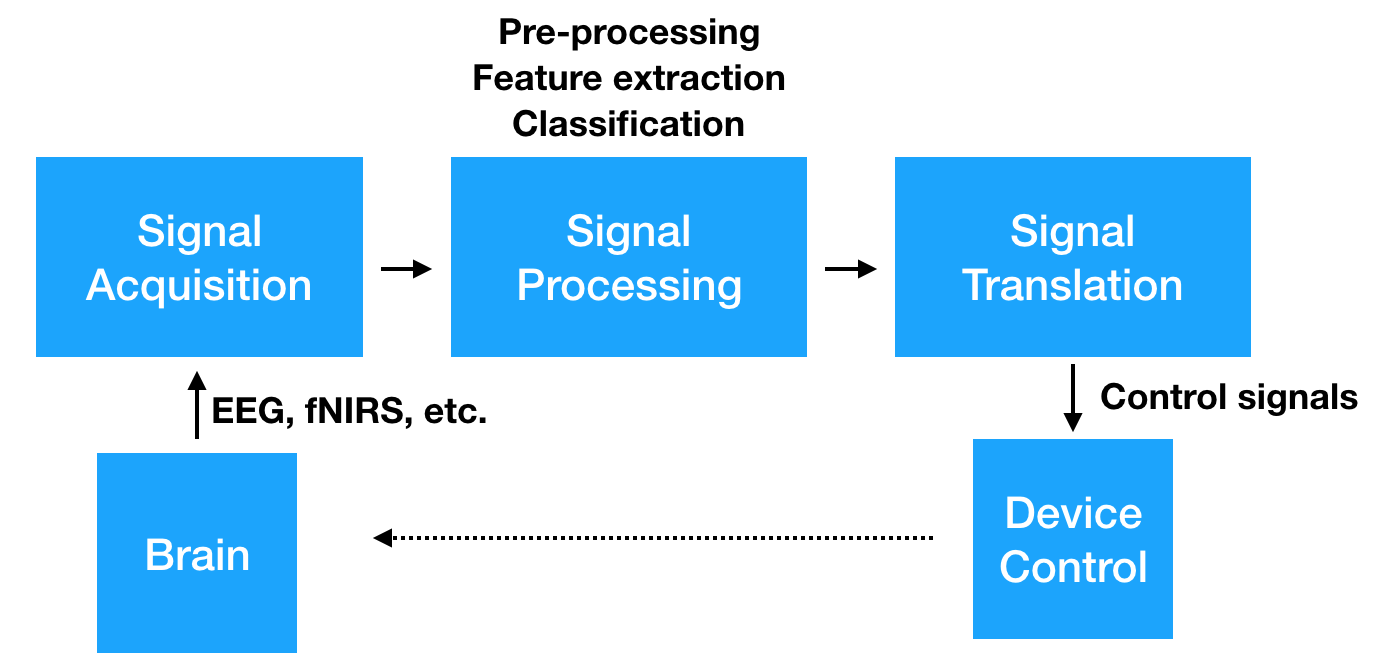
\includegraphics[width=0.5\linewidth]{image/bci}
	\caption{Basic procedure of a BCI}
\end{figure}
\end{frame}

\begin{frame}
\frametitle{Underlying Neural Processes}
\begin{itemize}
	\item All BCIs have to operate on observable effects of brain activity
	\item Except for fMRI and fNIRS, they operate on effects of neural firing processes
	\item EEG, MEG, and ECoG can only detect \textit{large-scale} neural dynamics
	\item For example, 50,000 neurons firing in near-synchrony
\end{itemize}
\end{frame}

\begin{frame}
\frametitle{Underlying Neural Processes}
\begin{itemize}
	\item Largest contributors to the EEG are the pyramidal cells
	\item Radially oriented in the cortex (orthgonal to the surface)
	\item Electromagnetic fields of co-aligned and co-activated neurons add up
	\item \url{https://www.youtube.com/watch?v=AIvlNNFQLEk}
\end{itemize}
	\begin{figure}
		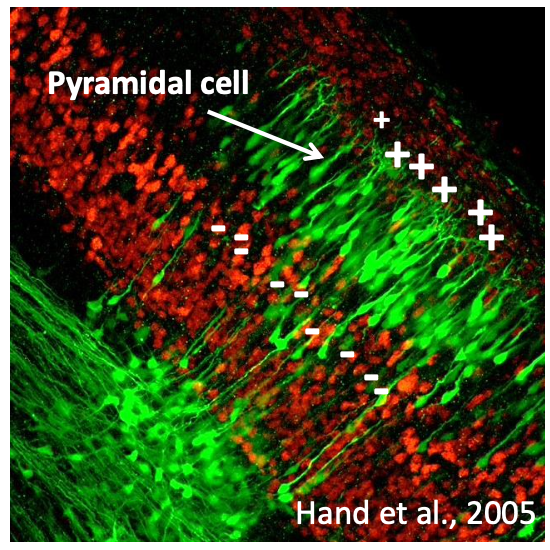
\includegraphics[width=0.3\linewidth]{image/pyra}
		\caption{Hand et al., 2005}
	\end{figure}
\end{frame}

\begin{frame}
\frametitle{Large-Scale Neural Processes}
\begin{itemize}
	\item When would 50,000 neurons fire near-synchronously?
	\begin{itemize}
		\item An external even triggers a cascade of related neural processes (e.g., in perception)
		\item An internal event triggers a cascade of related neural processes (e.g., a sudden aha!)
		\item Neural populations enter a synchronized steady-state firing pattern (e.g., idle oscillations)
	\end{itemize}
\end{itemize}
\end{frame}

\begin{frame}
\frametitle{Why BCI is so hard?} 
\begin{itemize}
	\item The field of BCI has been established since the 1960s - 1970s with a lot of promise.  However, contrary to the belief that "most obvious areas" are done (e.g., Neuralink), \textbf{BCI is still at its infancy.} 
	\item Most of the time,  BCI suffers from two key scientific challenges:
	\begin{enumerate}
		\item \textbf{Variability} - individuals variability in brain signals.  These variability is task-specific and user-specific.  Thus all BCI systems must be calibrated before they can be used.  Current research focuses on developing a transferable model of BCI that work across users.
		\item \textbf{Signal-to-noise ratio} - concerns the removal of artifacts while preserving the "weak" EEG signal.  Effective signal processing and machine learning is key here.  All approaches here are fundamentally statistical and computational.
	\end{enumerate}	 
\end{itemize}
\end{frame}

\begin{frame}
\frametitle{Three main types of BCI (Zander et al. 2009)} 
	\begin{enumerate}
		\item \textbf{Active} BCI:  A BCI of which users consciously control/manipulate their thoughts to control an application, e.g., \textit{motor imagery}
		\item \textbf{Reactive} BCI: A BCI of which output from brain activity arise from external stimulation, independent of users' conscious thoughts, e.g., \textit{P300}, \textit{SSVEP}
		\item \textbf{Passive} BCI: A BCI of which focused on utilizing our daily brain signals (without users' conscious thoughts) to enrich our daily life/interaction,  e.g. \textit{spectral analysis}
	\end{enumerate}	 
\end{frame}

\begin{frame}
\frametitle{BCI paradigms} 
BCI paradigms define how signals are being induced from the brain:
	\begin{itemize}
	\item \textbf{Motor Imagery}:  a dynamic state during which an individual mentally simulates a physical action
	\item \textbf{SSVEP}: steady state visually evoked potentials are signals that are natural responses to visual stimulation at specific frequencies
	\item \textbf{P300}: a positive deflection in the EEG signal that appears approximately 300 ms after the presentation of an attended stimulus
	\item \textbf{Spectral analysis}: analysis in terms of a spectrum of frequencies (e.g., alpha beta, gamma)
	\end{itemize}
\end{frame}

\begin{frame}
\frametitle{Motor imagery} 
\begin{figure}
	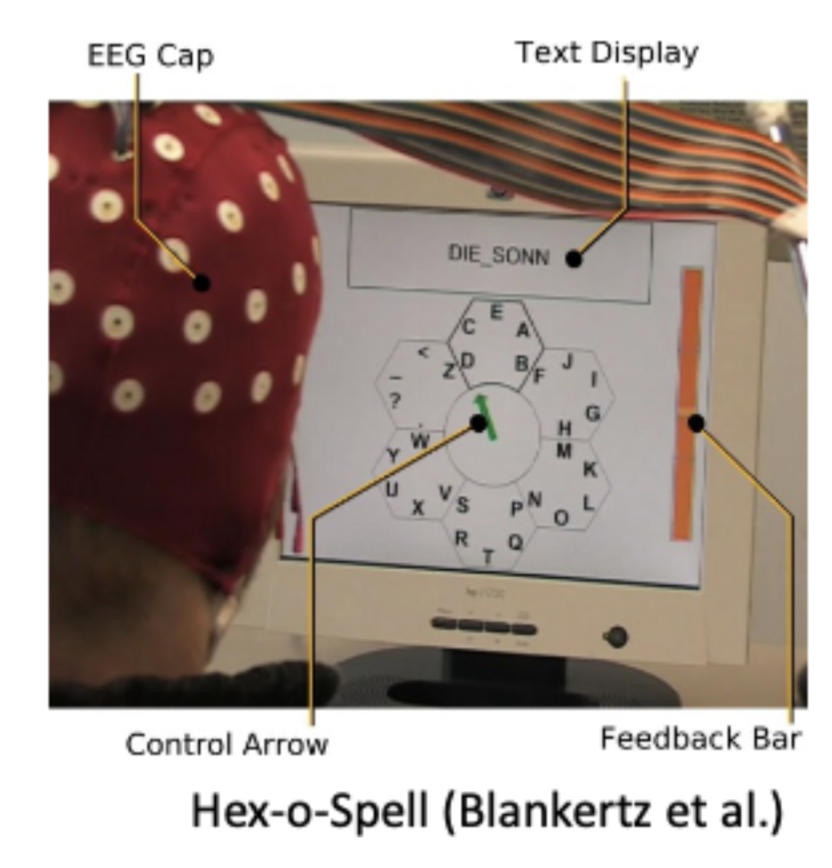
\includegraphics[width=0.5\linewidth]{image/mi1}
	\caption{Motor Imagery based speller}
\end{figure}
\end{frame}

\begin{frame}
\frametitle{Motor imagery} 
\begin{figure}
	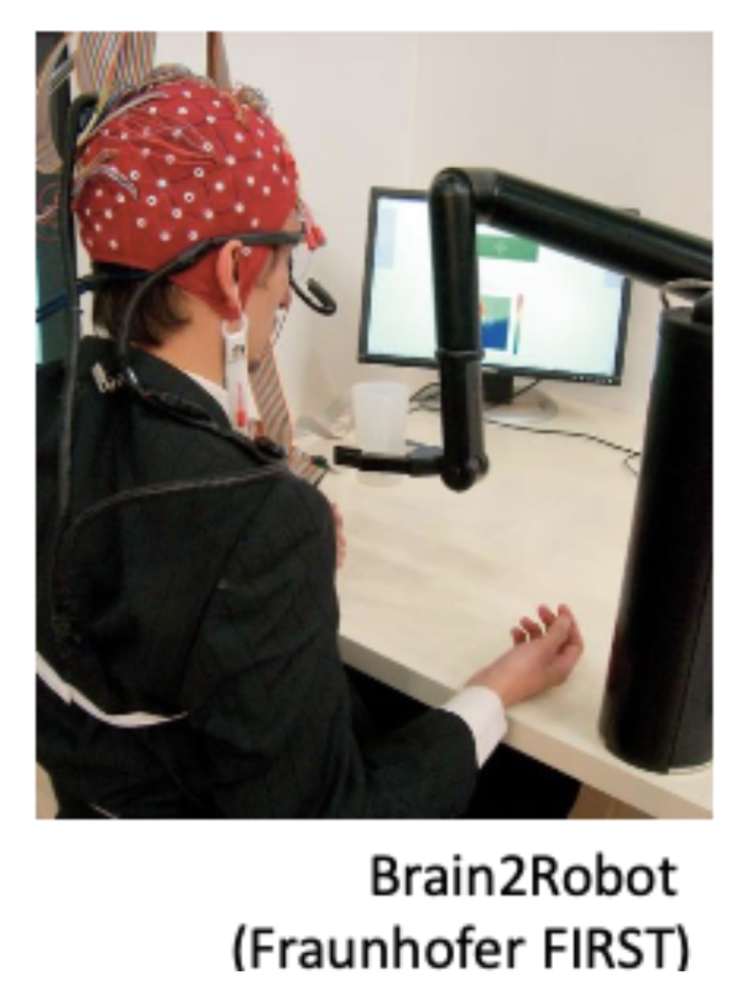
\includegraphics[width=0.4\linewidth]{image/mi2}
	\caption{Motor Imagery based prosthetic arm}
\end{figure}
\end{frame}

\begin{frame}
\frametitle{P300} 
\begin{figure}
	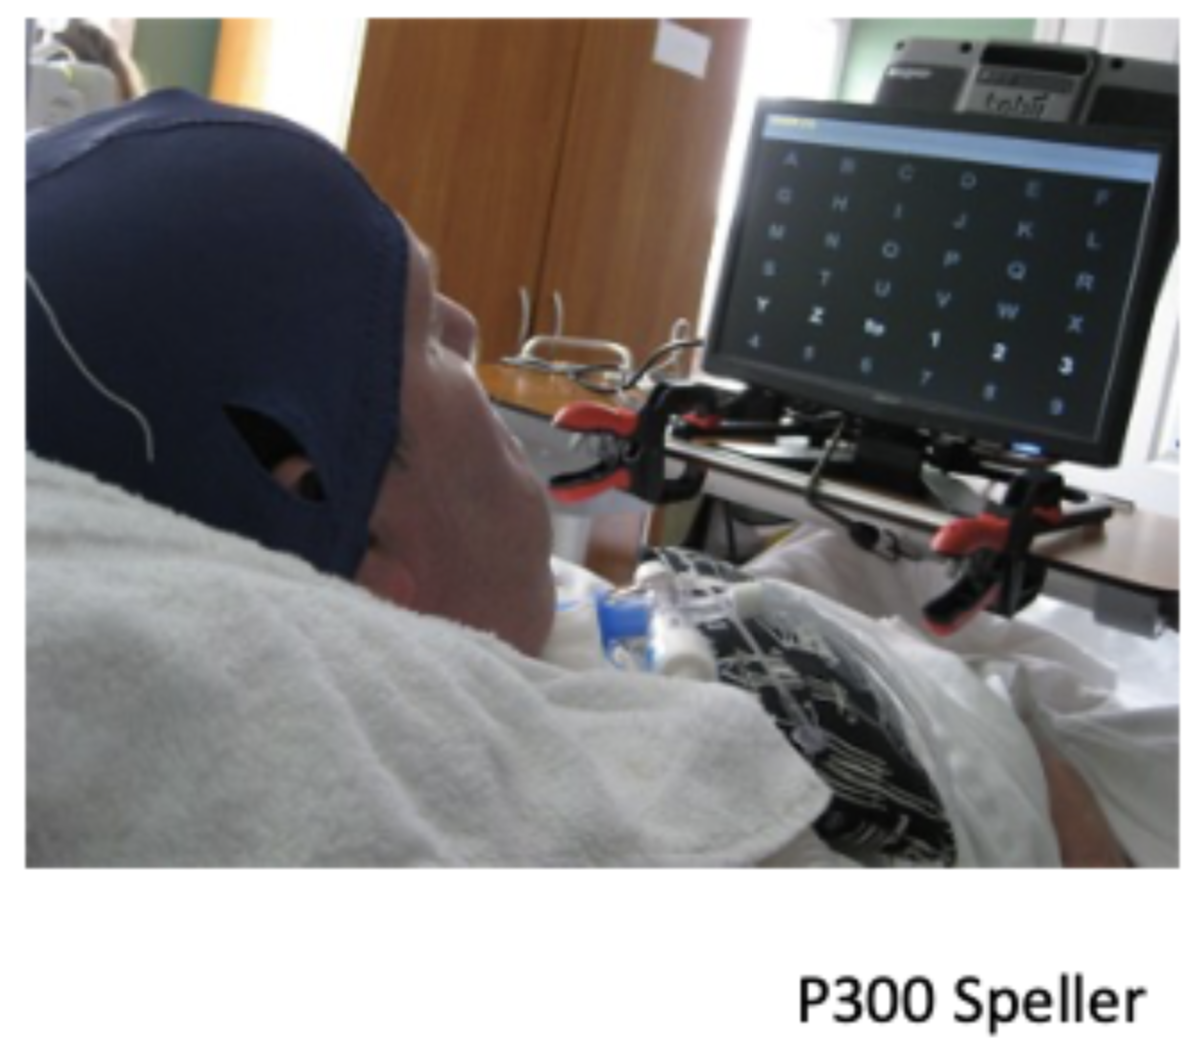
\includegraphics[width=0.4\linewidth]{image/p300}
	\caption{P300 speller}
\end{figure}
\centering
\url{https://www.youtube.com/watch?v=y3lGJVnSSsg}
\end{frame}

\begin{frame}
\frametitle{SSVEP} 
\begin{figure}
	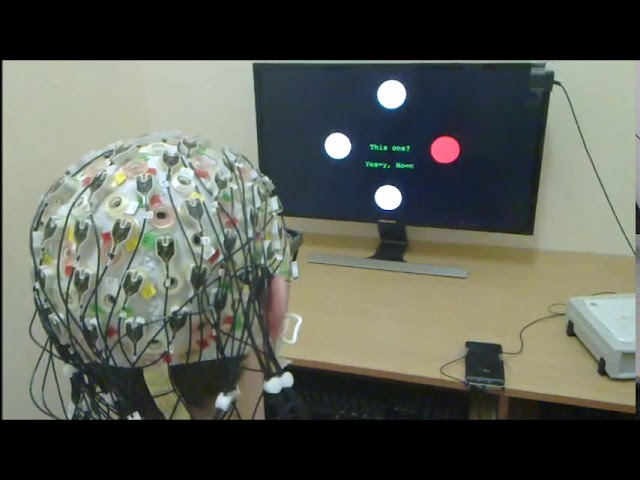
\includegraphics[width=0.4\linewidth]{image/ssvep}
	\caption{SSVEP}
\end{figure}
\centering
\url{https://www.youtube.com/watch?v=t96rl1SFHlI}
\end{frame}

\begin{frame}
\frametitle{Spectral analysis} 
\begin{figure}
	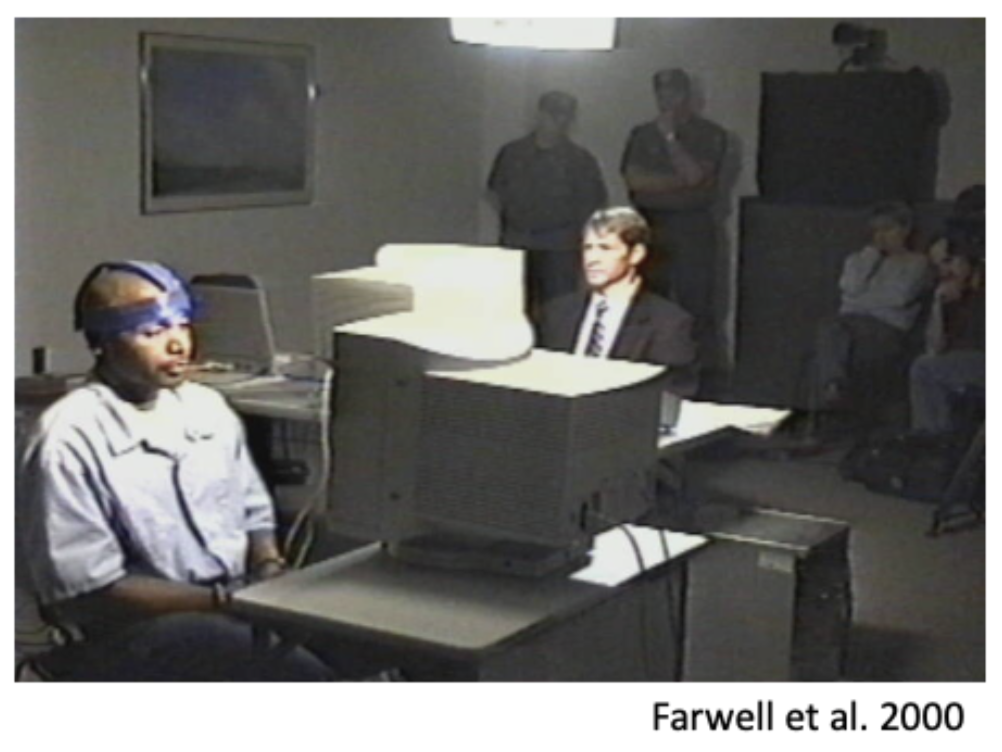
\includegraphics[width=0.7\linewidth]{image/s1}
	\caption{Lie detection}
\end{figure}
\end{frame}

\begin{frame}
\frametitle{Spectral analysis} 
\begin{figure}
	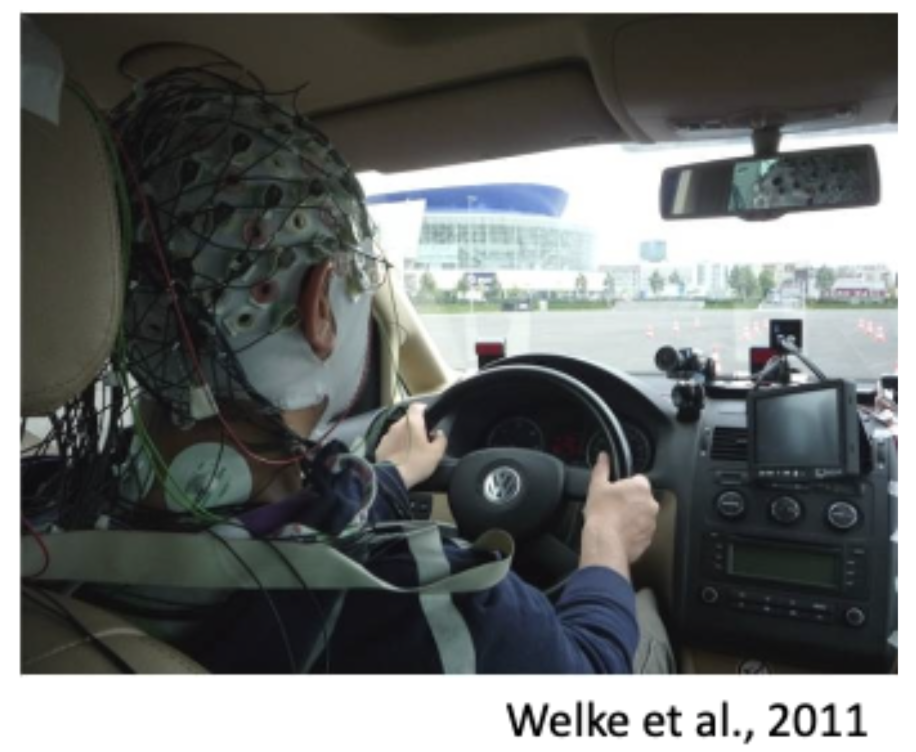
\includegraphics[width=0.6\linewidth]{image/s2}
	\caption{Cognitive load detection}
\end{figure}
\end{frame}

\begin{frame}
\frametitle{Future Applications}
\begin{itemize}
\item \textbf{Communication} - focuses on developing speller for locked-in patients so they can communicate with their caregivers.  FB is making a speller for normal people to type even faster!
\item \textbf{Control} - focuses on using BCI to controlling prostheses device, for home automation, for gaming and etc.
\item \textbf{Therapy/Rehabilitation} - focuses on using neurofeedback for rehabilitating users' attention or emotion. 
\item \textbf{Monitoring} - an area concerning affect/intent/cognitive state detection using the brain signals.  Workload, fatigue, breaking intent, lie detection are some example states. 
\item \textbf{Cross-Modal learning} - converting EEG to image/speech.  
\end{itemize}
\end{frame}

\begin{frame}
\footnotesize
\frametitle{Available tools}
\begin{itemize}
	\item \textbf{BioSig} - oldest open-source BCI toolboxes for offline processing (no GUI)
	\item \textbf{BCI2000} - written in C++ and mainly for online processing (acquisition, running experiments) but lack offline processing (e.g., algorithms)
	\item \textbf{OpenViBE} - written in C++;  gives a block programming (for non-programmers).  Requires Lua knowledge to extend/customize.
	\item \textbf{BCILAB} - matlab-based; lots of algorithms.  Requires Matlab knowledge to extend/customize.  Little support for acquisition systems but can tie to Lab Streaming Layer (LSL), a low-level technology that allow exchange of time series data between devices.
	\item \textbf{EEGLAB} - matlab-based; lots of algorithms.   Requires Matlab to extend/customize
	\item \textbf{MNE-python + other python libraries} - python-based; for programmers.  Lots of examples online.  Work well with other python libraries.  Requires python knowledge to extend/customize. 
\end{itemize}
\end{frame}

\section{EEG Analyses}

\subsection{Time-domain analyses}

\begin{frame}
\frametitle{Event-Related Potentials (ERPs)}
\begin{itemize}
	\item Averaging EEG activity relative to an event results in primarily event-induced activity (trial-to-trial variability averaged out)
\end{itemize}
	\begin{figure}
		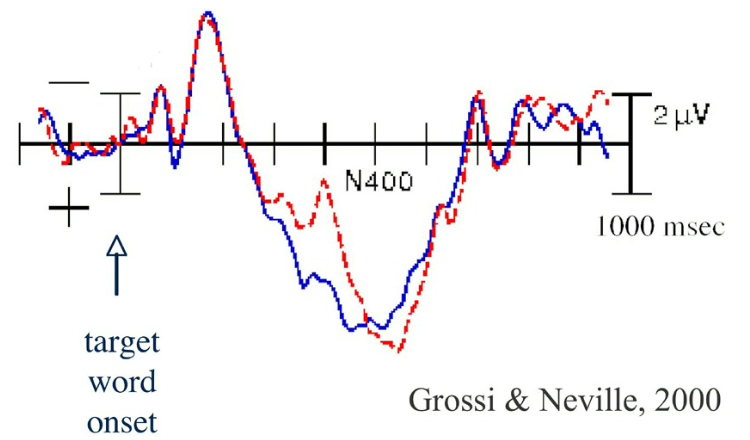
\includegraphics[width=0.7\linewidth]{image/erp}
		\caption{ERP of N400}
	\end{figure}
\end{frame}

\begin{frame}
\frametitle{Event-Related Potentials (ERPs)}
\begin{itemize}
	\item Single-trial ERPs are much harder to identify
\end{itemize}
	\begin{figure}
		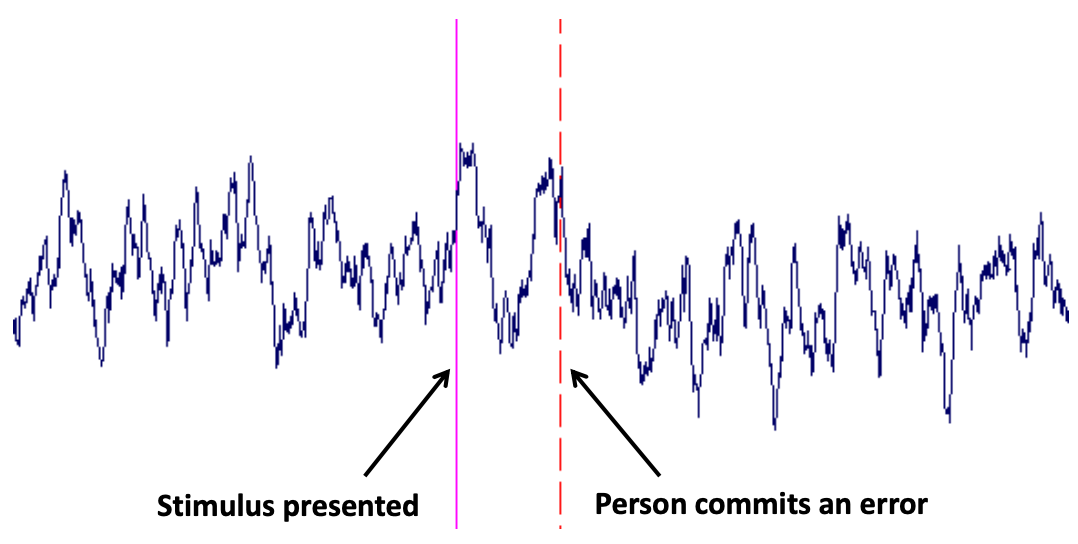
\includegraphics[width=0.8\linewidth]{image/erp2}
		\caption{Single-trial ERPs}
	\end{figure}
\end{frame}

\begin{frame}
\frametitle{Pros and Cons}
Pros:
\begin{itemize}
	\item Computationally simple
	\item Decades-old literature
	\item Used in P300 and N400
\end{itemize}
Cons:
\begin{itemize}
	\item Jittered and non-phase locked activities are lost
	\item Limited analysis possibilities (e.g., connectivity)
	\item Unclear biological mechanism
\end{itemize}
\end{frame}

\subsection{Frequency-domain analyses}

\begin{frame}
\frametitle{Frequency-domain analyses}
\begin{figure}
		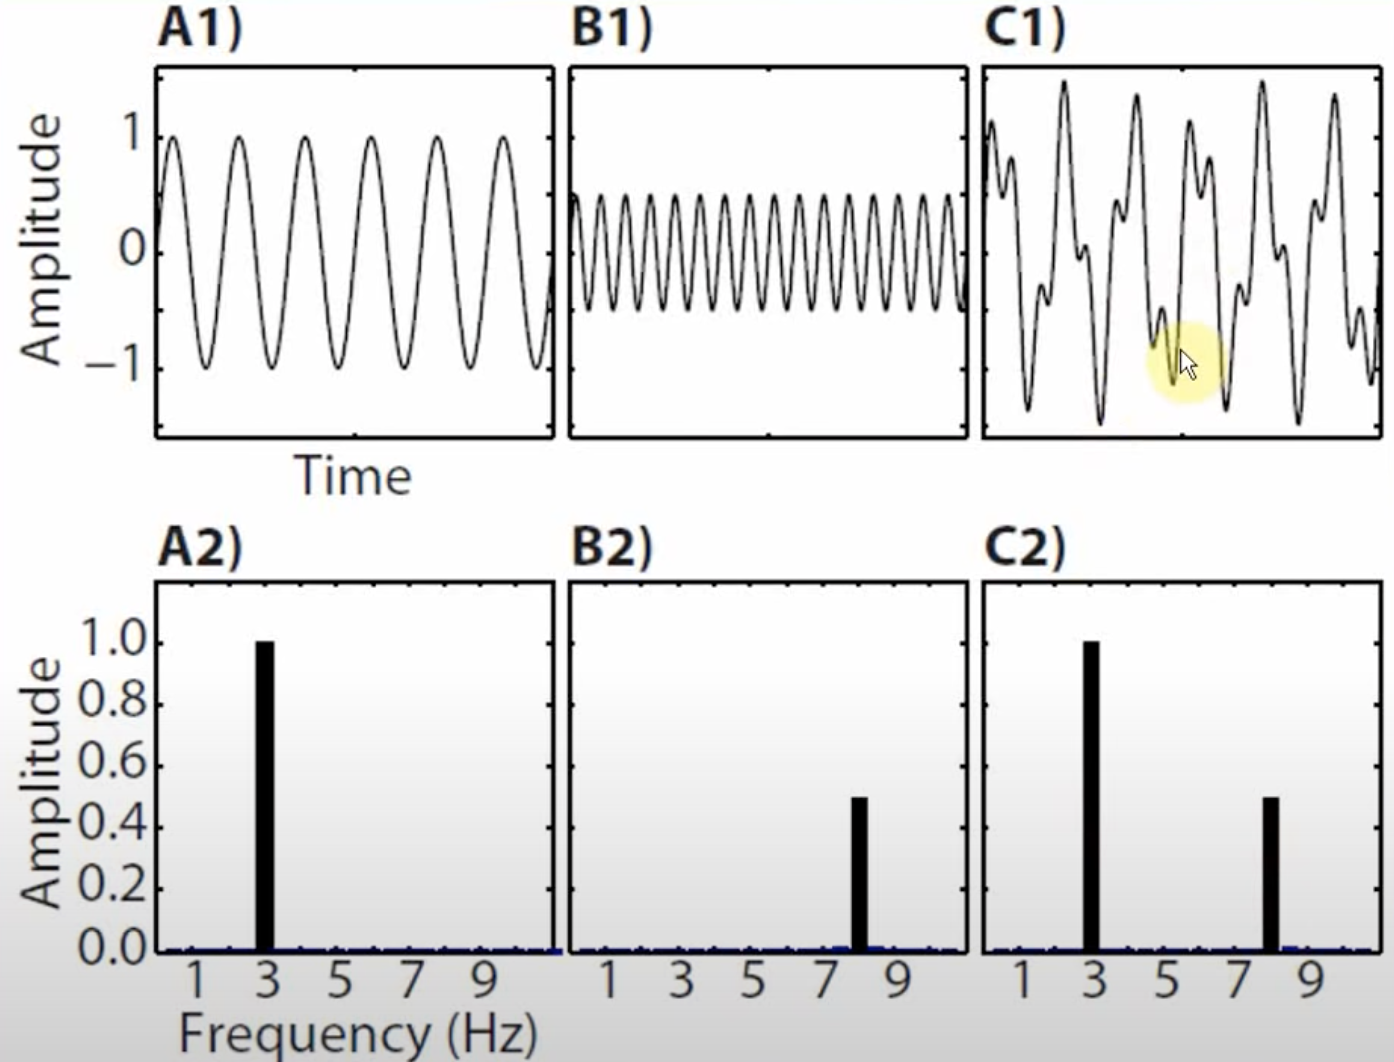
\includegraphics[width=0.7\linewidth]{image/frequency}
		\caption{Changing time to frequency domain}
\end{figure}
\end{frame}

\begin{frame}
\frametitle{Fourier Transform}
\begin{figure}
		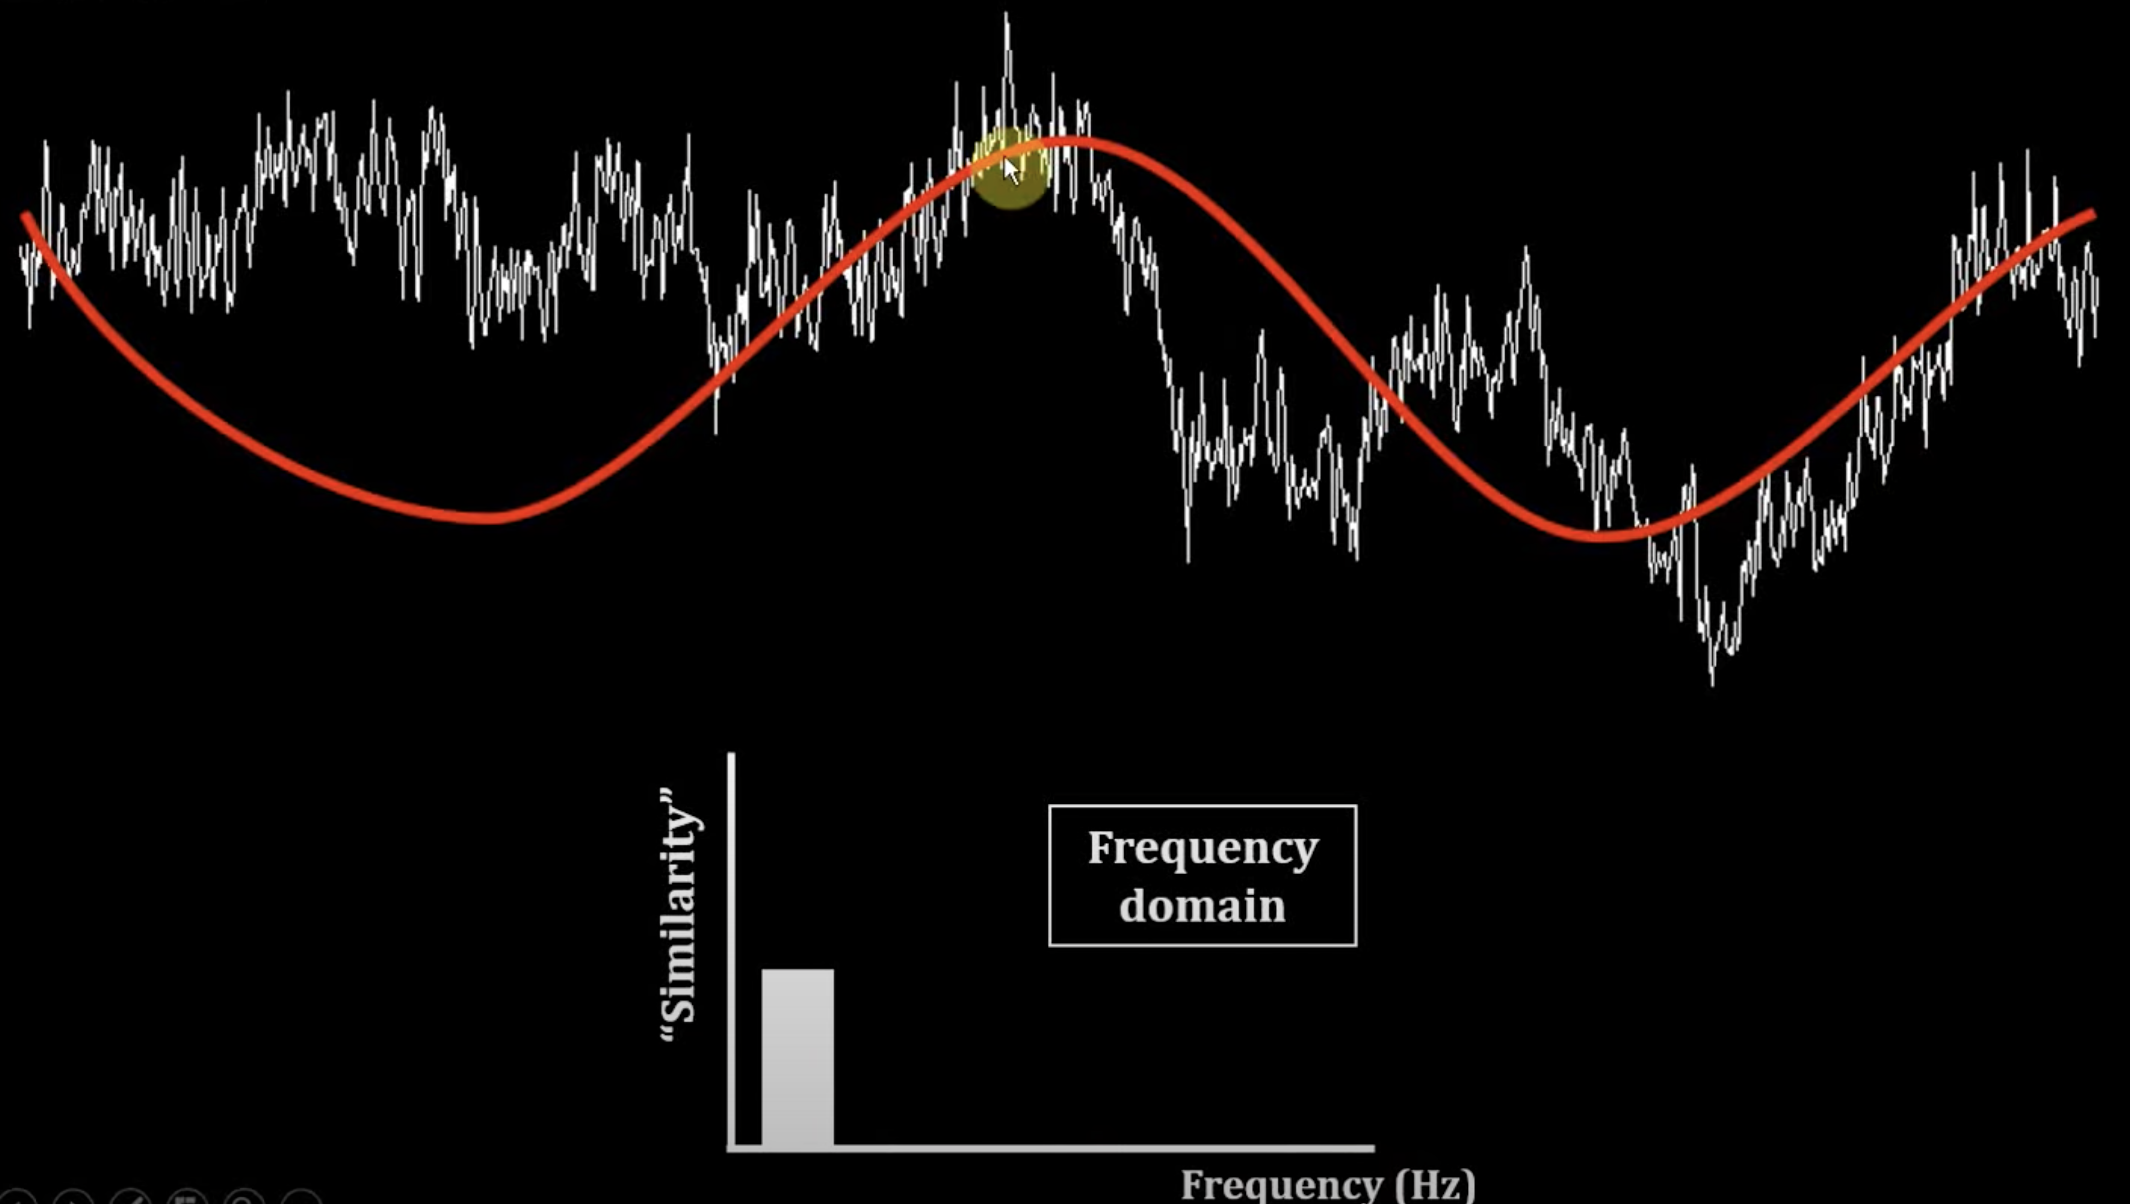
\includegraphics[width=0.7\linewidth]{image/ft}
		\caption{Dot product of particular sine wave with the EEG signal will give the corresponding similarity index.  For example, a sine wave of 2Hz dot product with the EEG will give the frequency component of 2Hz.}
\end{figure}
\end{frame}

\begin{frame}
\frametitle{Pros and Cons}
Pros:
\begin{itemize}
	\item Computationally fast
	\item Ubiquitous in science and engineering
	\item Useful for oscillatory processes, e.g.,  delta (0-4Hz), theta (4-7Hz), alpha (8-13Hz), beta(12-30Hz), and gamma(25-100Hz)
	\item Used in SSVEP, emotion recognition, cognition recognition
\end{itemize}
Cons:
\begin{itemize}
	\item Lost time information
	\item Only good for stationary data.  Is EEG stationary?
\end{itemize}
\end{frame}

\subsection{Time-frequency domain analyses}

\begin{frame}
\frametitle{Time-frequency domain analyses}
\begin{figure}
		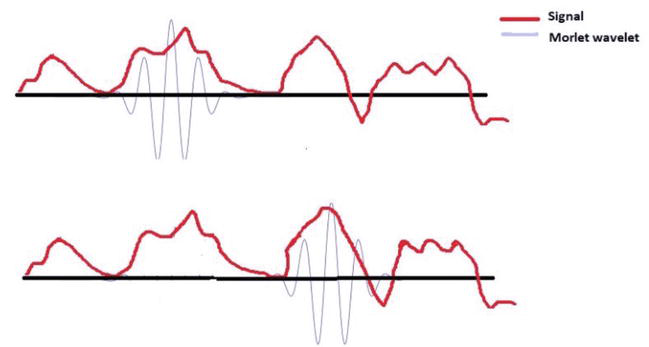
\includegraphics[width=0.7\linewidth]{image/wt}
		\caption{Instead of using a never ending sine wave, we can create a specific wavelet that captures only a specific time window.}
\end{figure}
\end{frame}

\begin{frame}
\frametitle{Time-frequency domain analyses}
\begin{figure}
		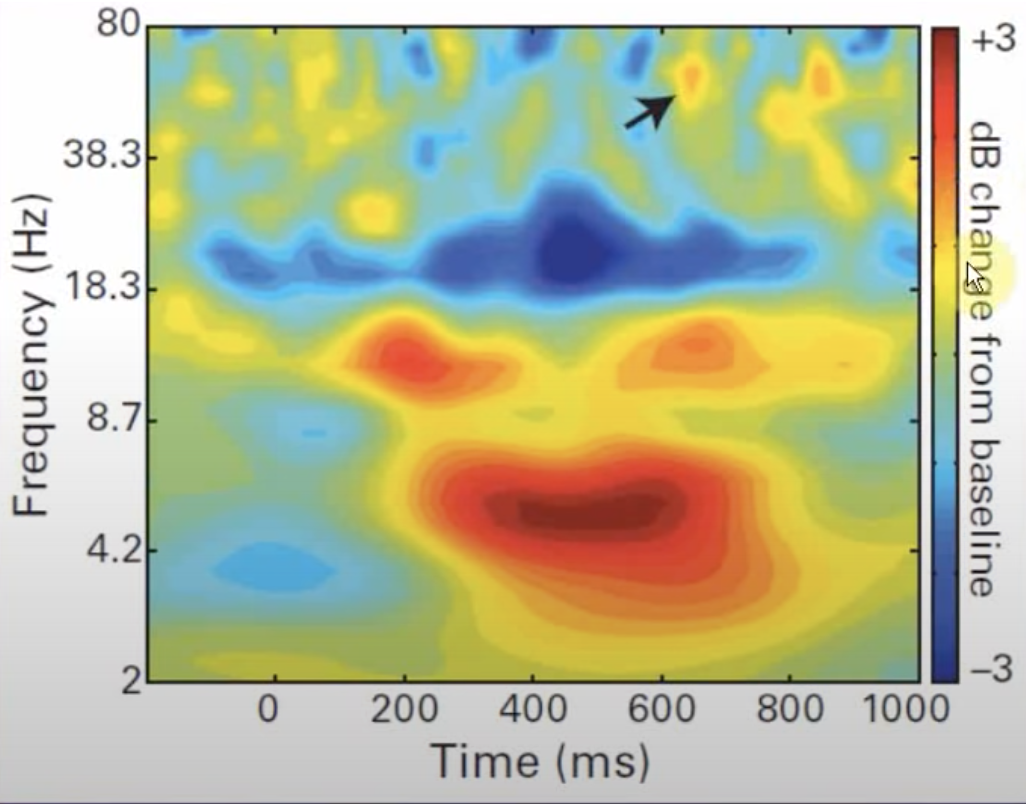
\includegraphics[width=0.6\linewidth]{image/spectrogram2}
		\caption{This will result in a spectrogram with both time and frequency information.}
\end{figure}
\end{frame}


\begin{frame}
\frametitle{Time-frequency domain analyses}
\begin{figure}
		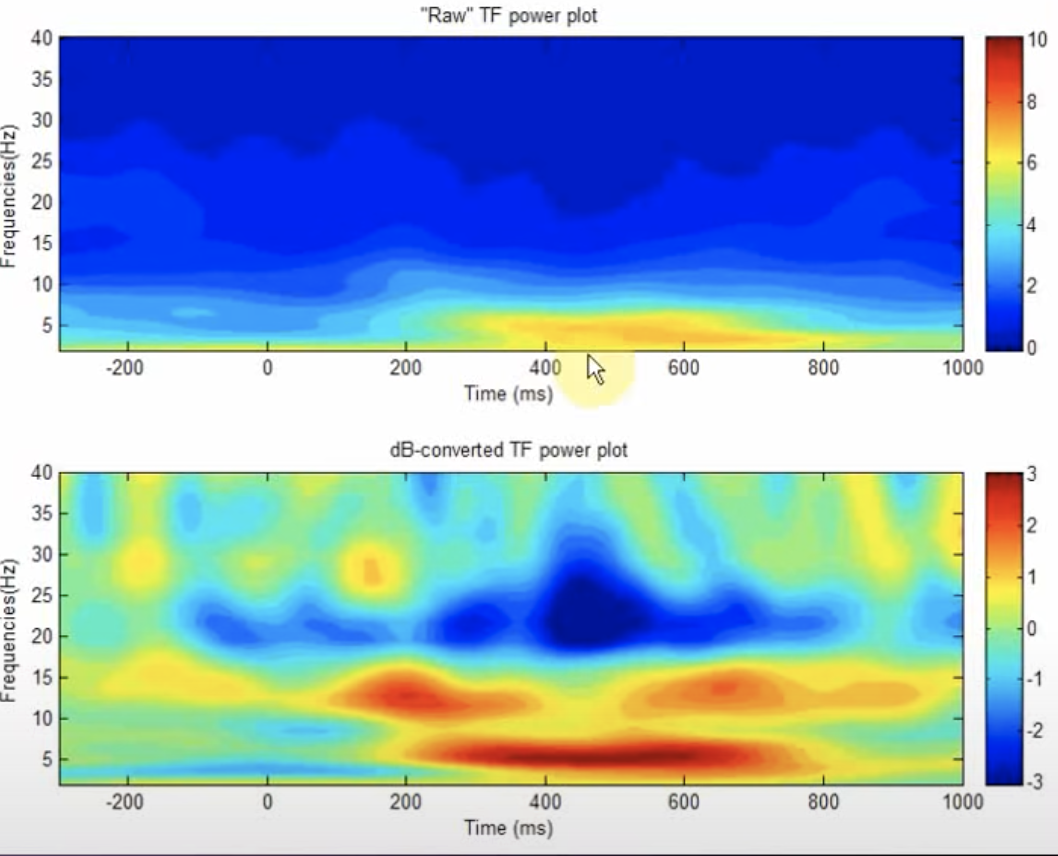
\includegraphics[width=0.6\linewidth]{image/normalization}
		\caption{Often wise to perform baseline normalization.  It transforms all data to same scale, disentangle task-related from background activity, and more like to be normally distributed thus good for classification.}
\end{figure}
\end{frame}

\begin{frame}
\frametitle{Pros and Cons}
Pros:
\begin{itemize}
	\item Almost the best..Thus common neural network often transform EEG to spectrograms first, and then use CNN
\end{itemize}
Cons:
\begin{itemize}
	\item Reduced temporal precision but it is a parameter we can fine tune....
\end{itemize}
\end{frame}

\subsection{Spatial Analyses}

\begin{frame}
\frametitle{Spatial Filters}
\begin{itemize}
	\item Transform a multi-channel signal $X(n)$ such that $Y(n)$ depends only on $X(n)$; most spatial filters are linear, i.e., $Y(n) = MX(n)$ for some matrix $M$
	\item Linear spatial filters can approximately invert volume conduction and remap channel signals to approximate source signals - this is the main use in BCIs
	\item Examples: Re-referencing, Surface Laplacian, Independent Component Analysis (CIA), Common Spatial Patterns (CSP)
\end{itemize}
\end{frame}
%
%\begin{frame}
%\frametitle{ICA}
%\begin{figure}
%	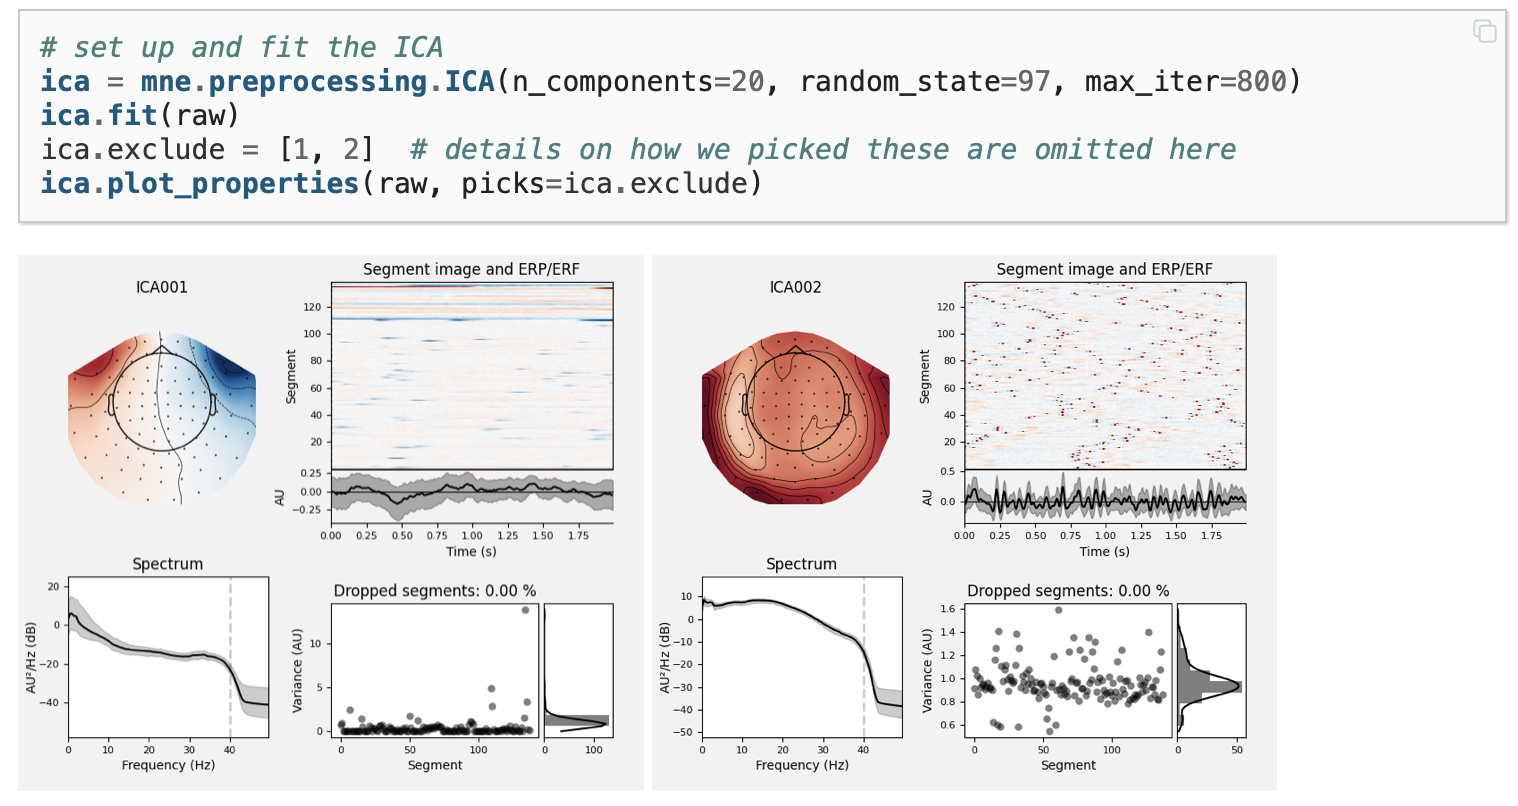
\includegraphics[width=0.8\linewidth]{image/ica2}
%	\caption{Independent Component Analysis}
%\end{figure}
%\end{frame}

\begin{frame}
\frametitle{Common Spatial Patterns}
\begin{itemize}
	\item Spatial filters designed to recover motor-cortex source activity, calculated via the Common Spatial Patterns algorithm
\end{itemize}
\begin{figure}
	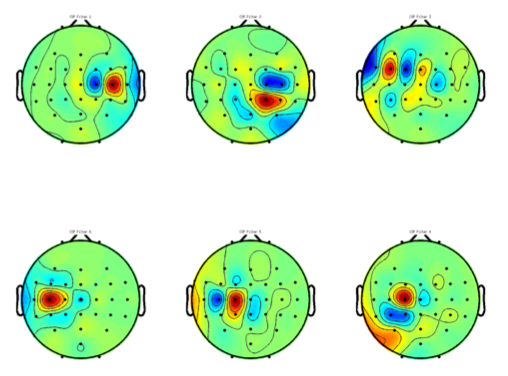
\includegraphics[width=0.6\linewidth]{image/sfilter}
	\caption{Common Spatial Patterns}
\end{figure}
\end{frame}

\begin{frame}
\frametitle{Spatial Filters vs. Forward Projections}
\begin{itemize}
	\item Spatial filters are not the same as forward project maps of some source signal - they are the inverse operation
\end{itemize}
\begin{figure}
	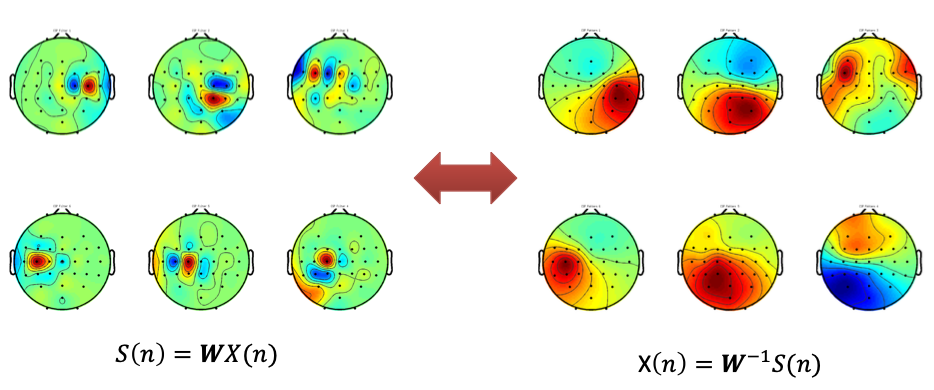
\includegraphics[width=0.8\linewidth]{image/sfilter2}
	\caption{Inverse operation of one another}
\end{figure}
\end{frame}

\begin{frame}
\frametitle{Common Spatial Filters}
\begin{figure}
	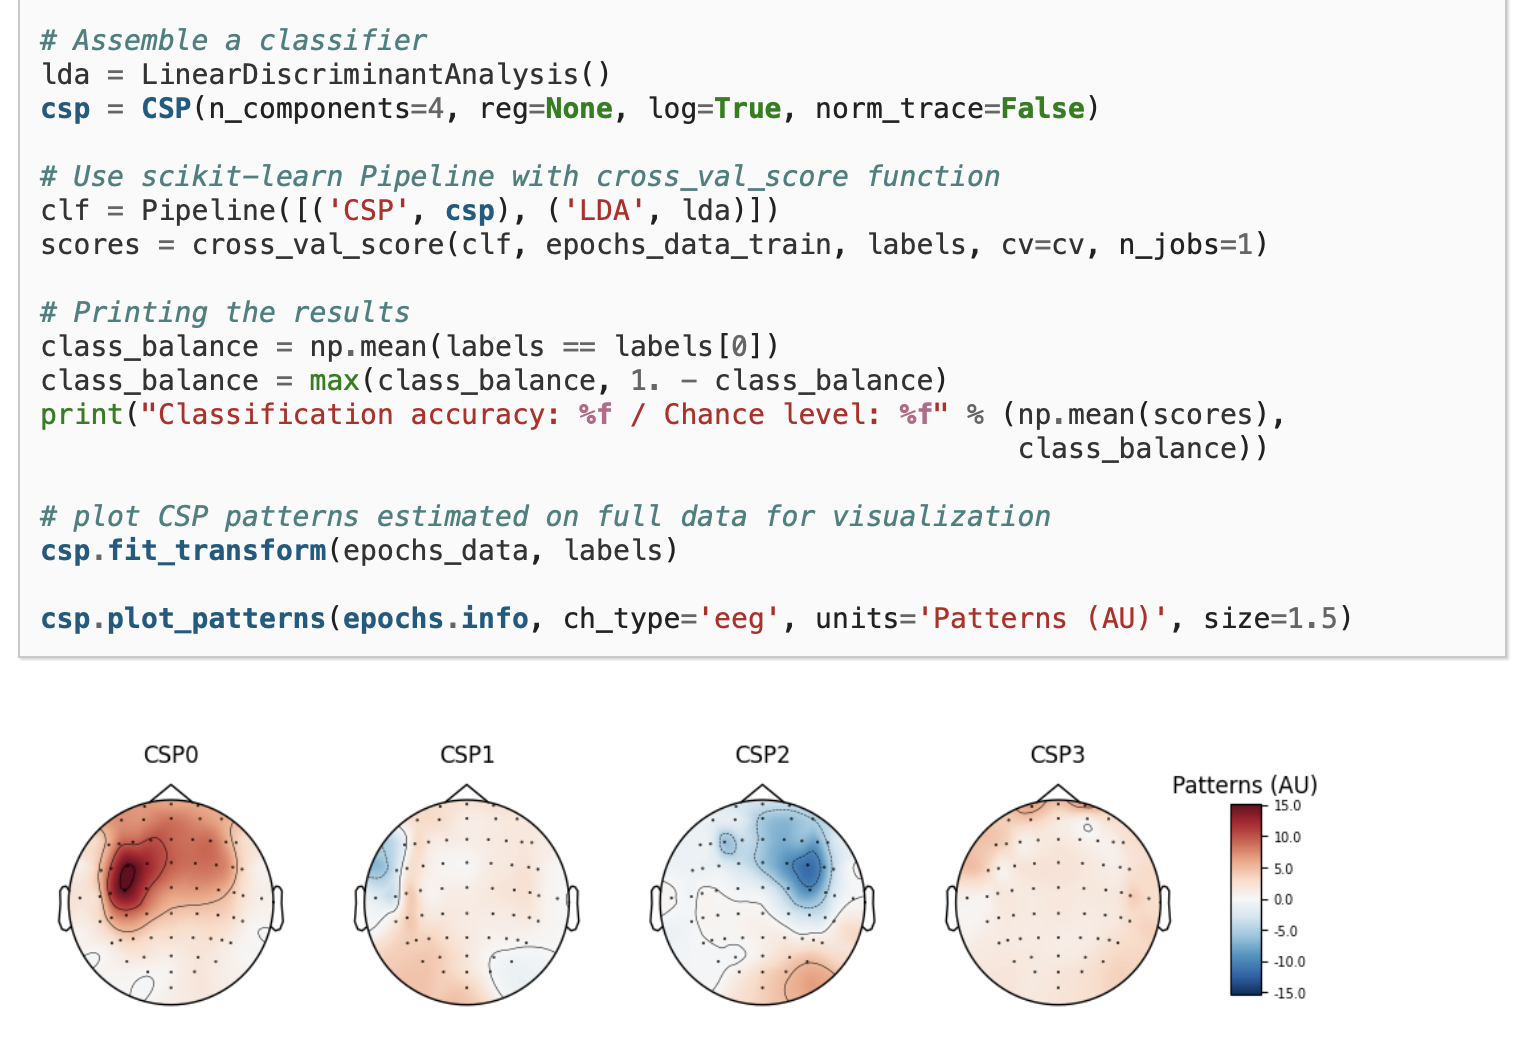
\includegraphics[width=0.7\linewidth]{image/csp}
	\caption{Common Spatial Filters}
\end{figure}
\end{frame}

\subsection{Topological Analyses}

\begin{frame}
\frametitle{Topological Analyses}
\begin{itemize}
	\item Topological analyses create scalp maps that allow for rough source localization
	\item Topological analyses are NOT source localization
\end{itemize}
	\begin{figure}
		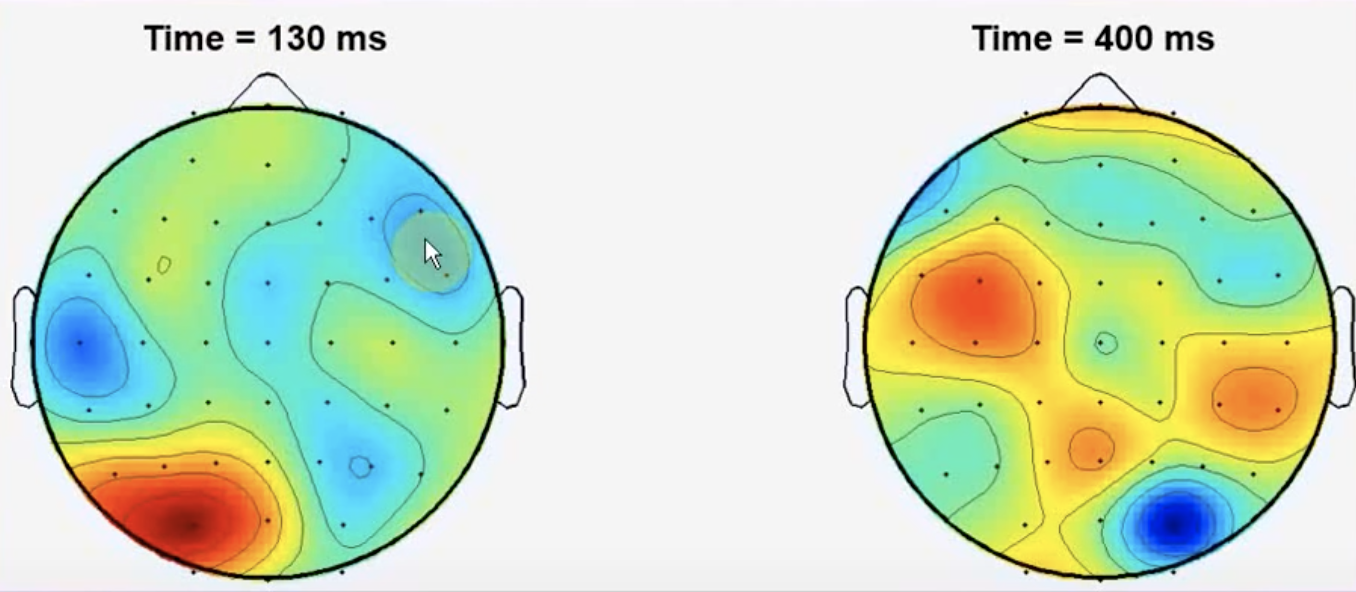
\includegraphics[width=0.7\linewidth]{image/scalpmap2}
		\caption{Left: Likely the participants are looking using the right eye; Right: Likely the participants are using the right hand to click.}
	\end{figure}
\end{frame}

\begin{frame}
\frametitle{More Scalp Maps}
	\begin{figure}
		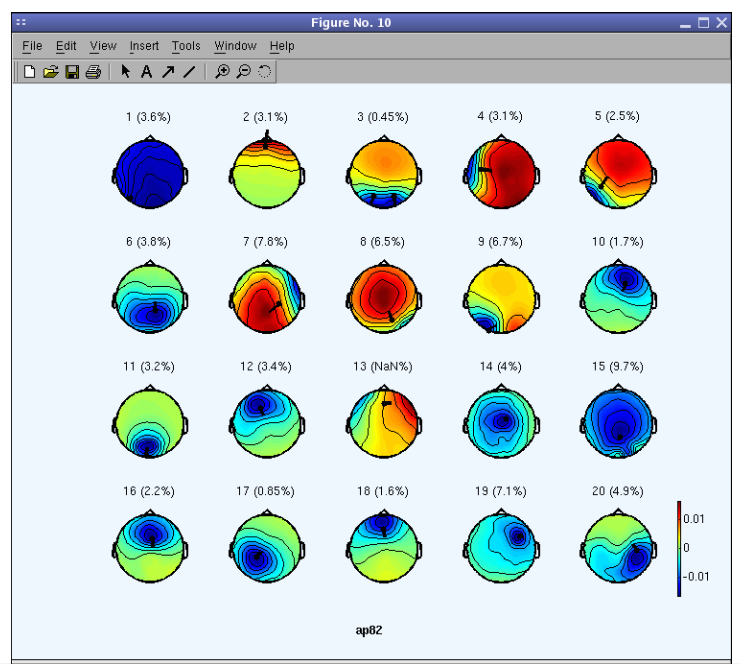
\includegraphics[width=0.5\linewidth]{image/scalpdipole}
		\caption{Scalp maps}
	\end{figure}
\end{frame}

\begin{frame}
\frametitle{Python MNE with scalp maps}
	\begin{figure}
		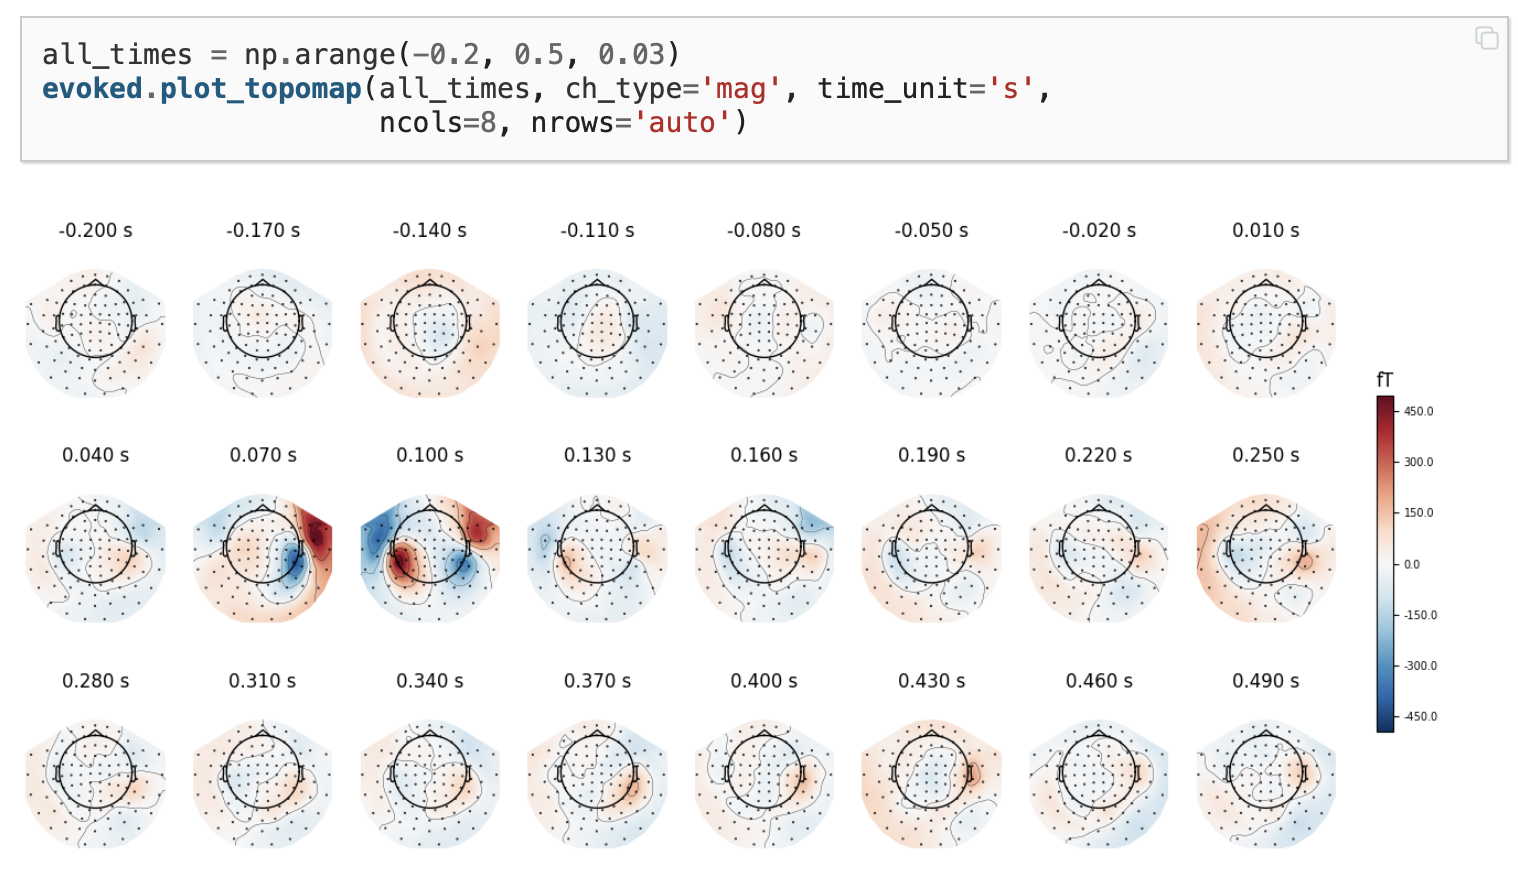
\includegraphics[width=0.8\linewidth]{image/scalp}
		\caption{Plot evoked topographies using MNE}
	\end{figure}
\end{frame}

\subsection{Source Localization}

%
%\begin{frame}
%\frametitle{Signal Detectability}
%\footnotesize
%\begin{itemize}
%	\item Root cause might not be directly observable (e.g., dopaminergic system, deep brain structures, few neurons)
%	\item Widely scattered neural populations are unlikely to exhibit synchrony (unless connected by fiber tracts)
%	\item Spatially compact populations are more likely to have coordinated timing
%	\item Electromanetic fields can cancel each other out (e.g., in the Amygdala)
%\end{itemize}
%	\begin{figure}
%		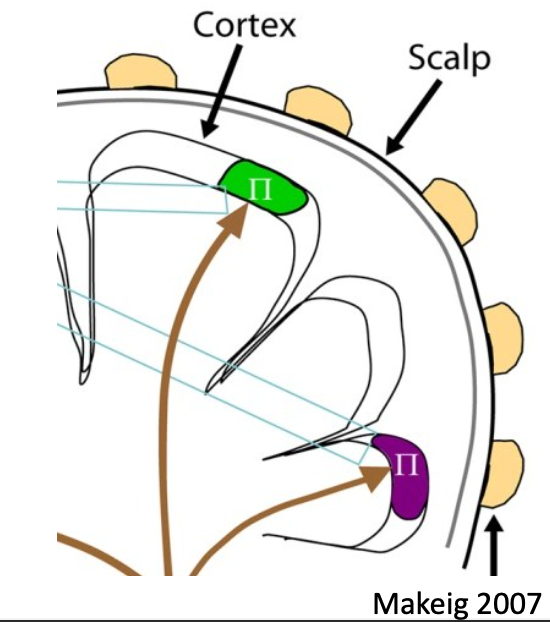
\includegraphics[width=0.3\linewidth]{image/makeig}
%		\caption{Makeig 2007}
%	\end{figure}
%\end{frame}

\begin{frame}
\frametitle{Volume Conduction}
\begin{itemize}
	\item Neural activity is conducted through the brain volume to the scalp which is instantaneous, and characterized by a electromagnetic field
	\item Volume conduction is linear, thus each sensor measures a (weighted) sum of each neuron's activity
\end{itemize}
	\begin{figure}
		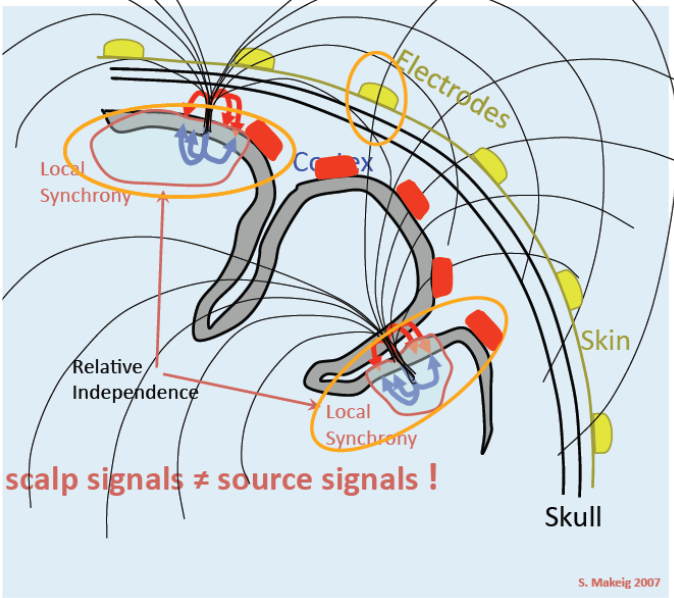
\includegraphics[width=0.4\linewidth]{image/firing}
		\caption{Neural activity}
	\end{figure}
\end{frame}

\begin{frame}
\frametitle{Volume Conduction}
\begin{itemize}
	\item Note: the point-spread function from a source patch to the scalp is extremely broad
\end{itemize}
	\begin{figure}
		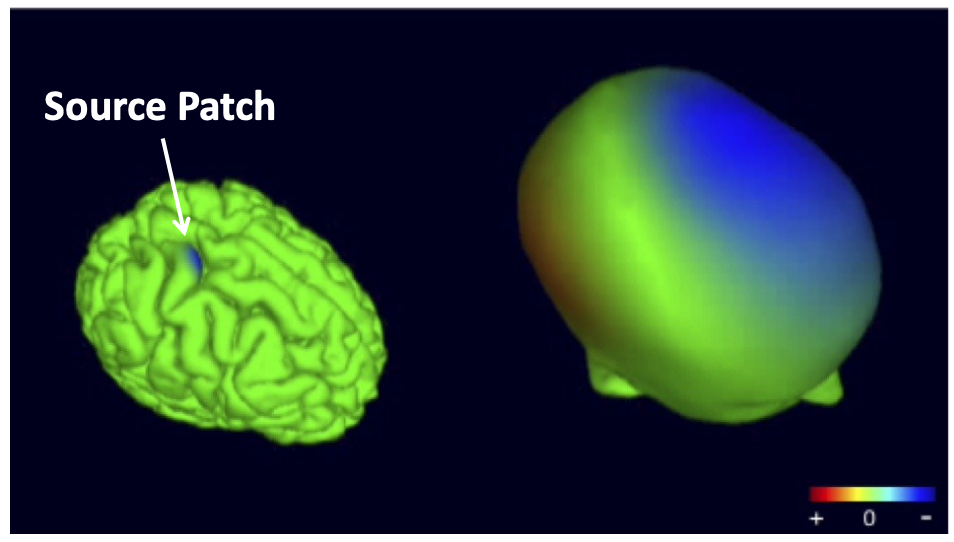
\includegraphics[width=0.7\linewidth]{image/source}
		\caption{Akalin Acar et al., 2011}
	\end{figure}
\end{frame}

\begin{frame}
\frametitle{Dipole Fitting}
\begin{itemize}
	\item Electromagnetic field sustained by a compact collection of neurons can be modeled as a single equivalent dipole
	\item This facilitates localization of the field source
\end{itemize}
	\begin{figure}
		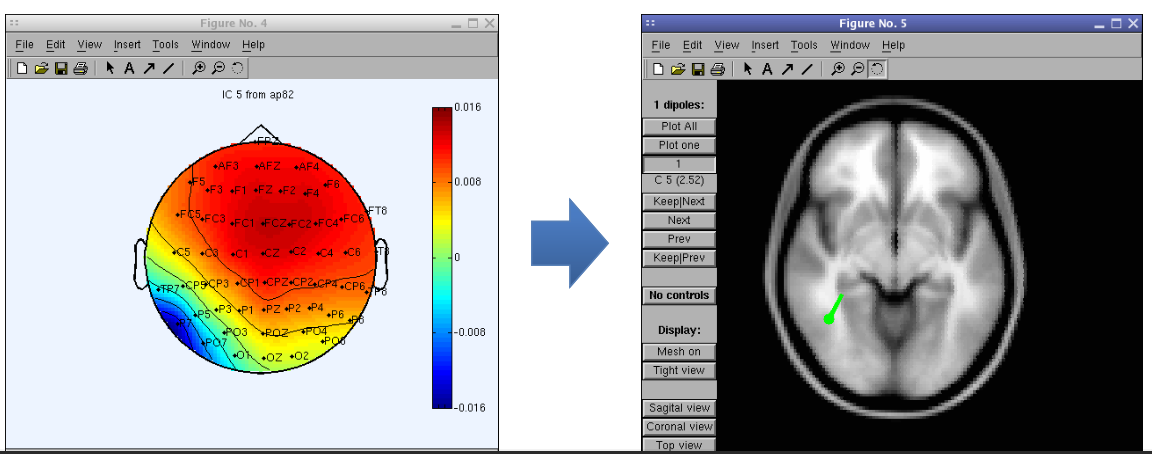
\includegraphics[width=0.8\linewidth]{image/dipole}
		\caption{Source localization}
	\end{figure}
\end{frame}

\begin{frame}
\frametitle{Dipole Fitting}
	\begin{figure}
		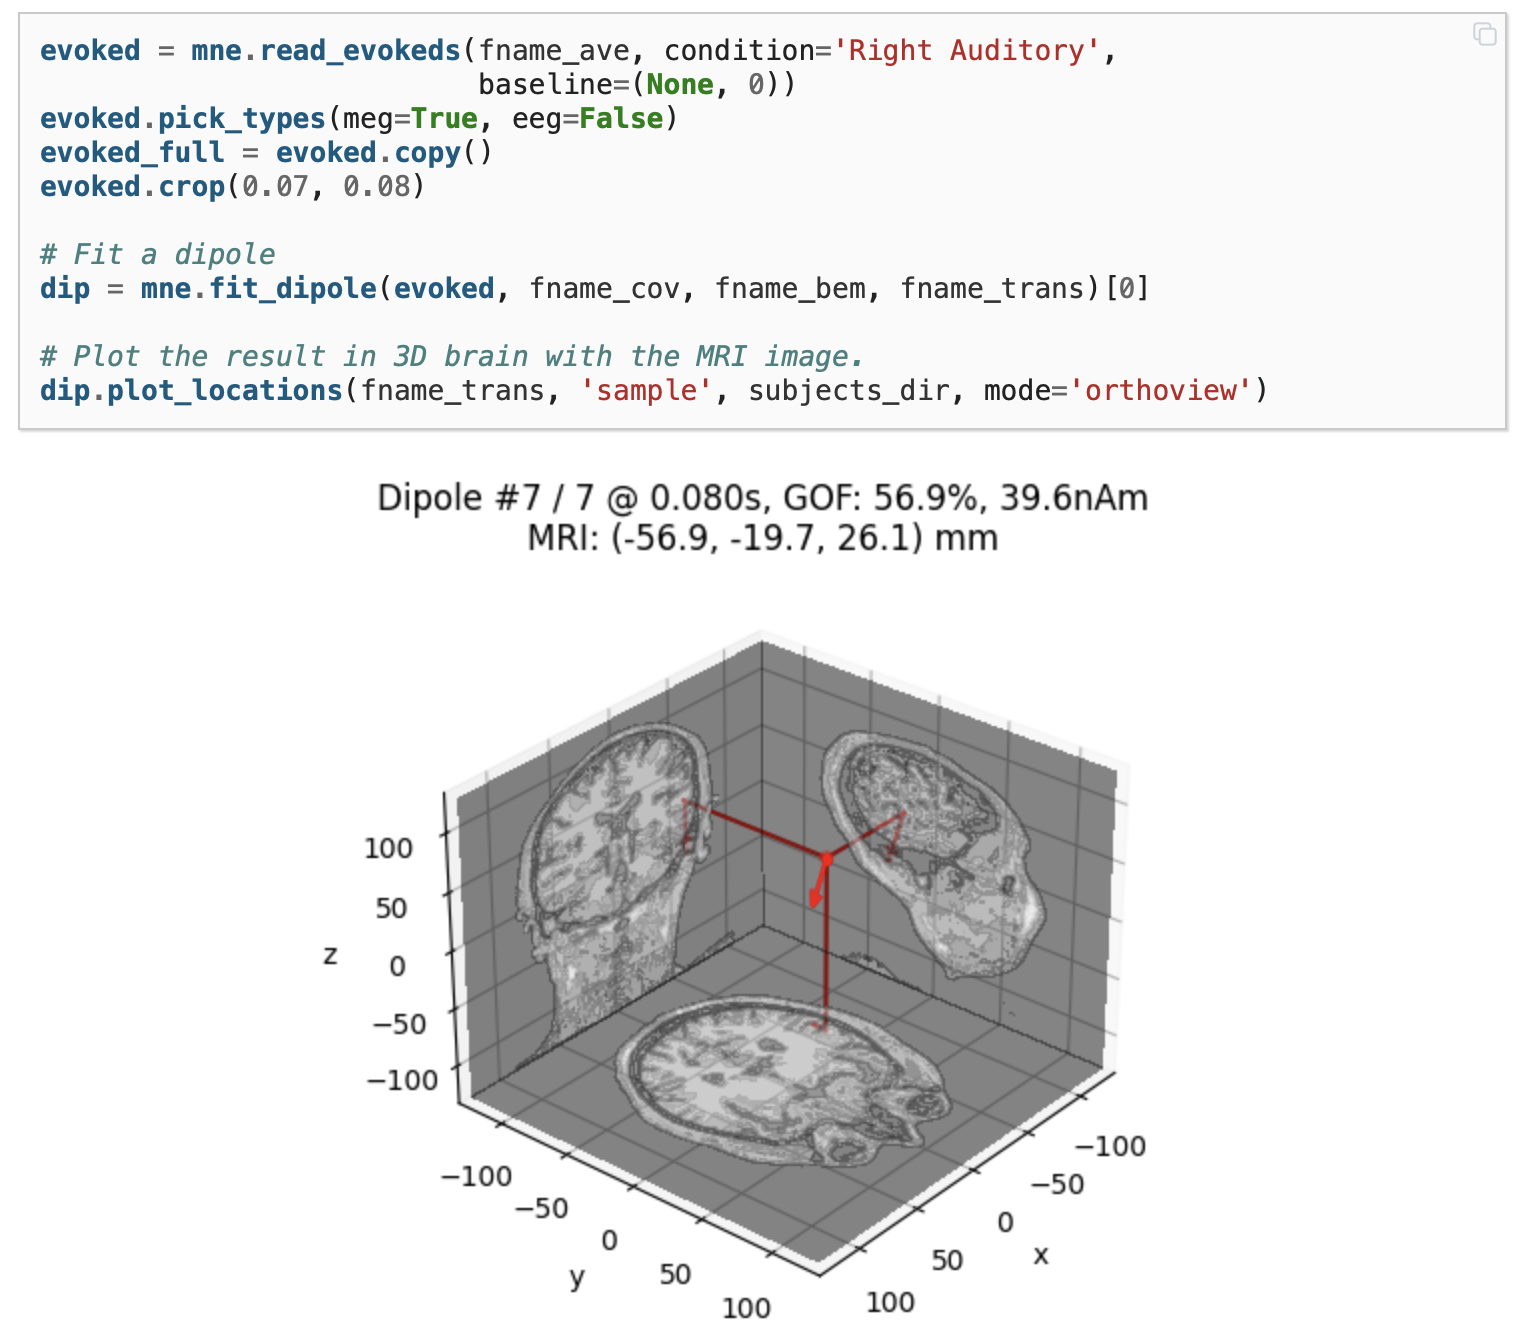
\includegraphics[width=0.7\linewidth]{image/dipolefitting}
		\caption{Dipole fitting using MNE}
	\end{figure}
\end{frame}

\begin{frame}
\frametitle{Dipole Modeling Problems}
\begin{itemize}
	\item High-quality fits are hard to achieve
	\begin{itemize}
		\item Requires knowledge about sensor locations
		\item Require assumptions about conductivities of scalp, skull, cerebrospinal fluid (CSF), brain tissue
		\item Requires knowledge of the folding of the cortex (candidate dipoles) unless simplistic spherical model is used
		\item Some brain tissues has anisotropic conductance (white matter)
		\item Scalp maps are usually not perfect (arise from data processing) - fit accuracy suffers
		\item Scalp maps can be a sum of multiple dipole sources - requires a distributed source model
	\end{itemize}
\end{itemize}
\end{frame}

\begin{frame}
\frametitle{Distributed Source Modeling}
\begin{itemize}
	\item Allow to recover and image distributed cortical support of given scalp maps
\end{itemize}
	\begin{figure}
		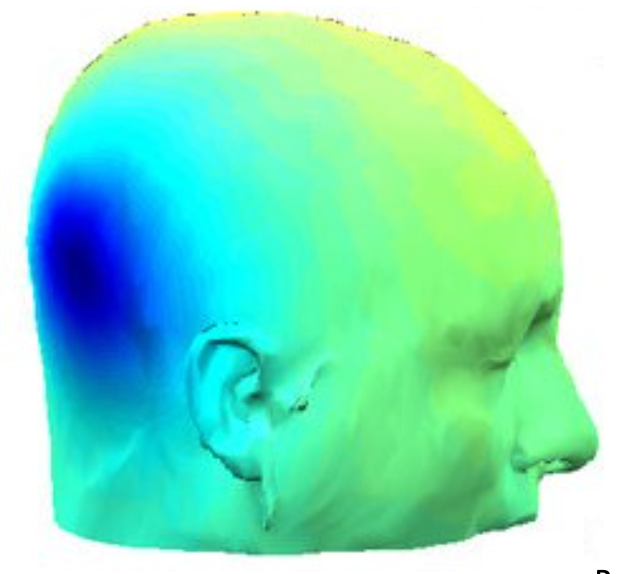
\includegraphics[width=0.5\linewidth]{image/dsm}
		\caption{Ray Ramirez (Scholarpedia)}
	\end{figure}
\end{frame}

\begin{frame}
\frametitle{Distributed Source Modeling}
\begin{itemize}
	\item Wide range of methodologies and underlying assumptions (sLORETA, Beamforming, Sparse Bayesian Learning, ...)
	\item Prone to finding only locally optimal solutions
\end{itemize}
	\begin{figure}
		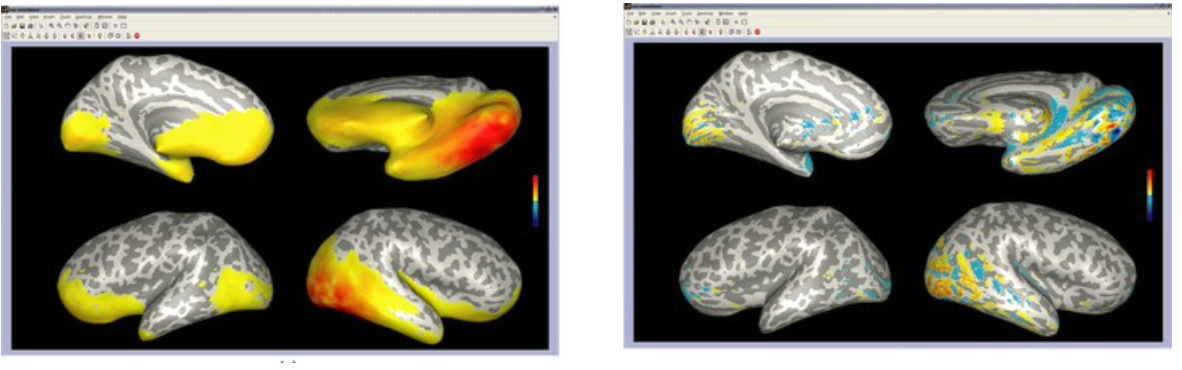
\includegraphics[width=0.8\linewidth]{image/dsm2}
		\caption{LCMV Beamforming (Left), Anatomically Constrained Beamforming (Right)}
	\end{figure}
\end{frame}

\begin{frame}
\frametitle{Distributed Source Modeling}
\begin{itemize}
	\item Wide range of methodologies and underlying assumptions (sLORETA, Beamforming, Sparse Bayesian Learning, ...)
	\item Prone to finding only locally optimal solutions
\end{itemize}
	\begin{figure}
		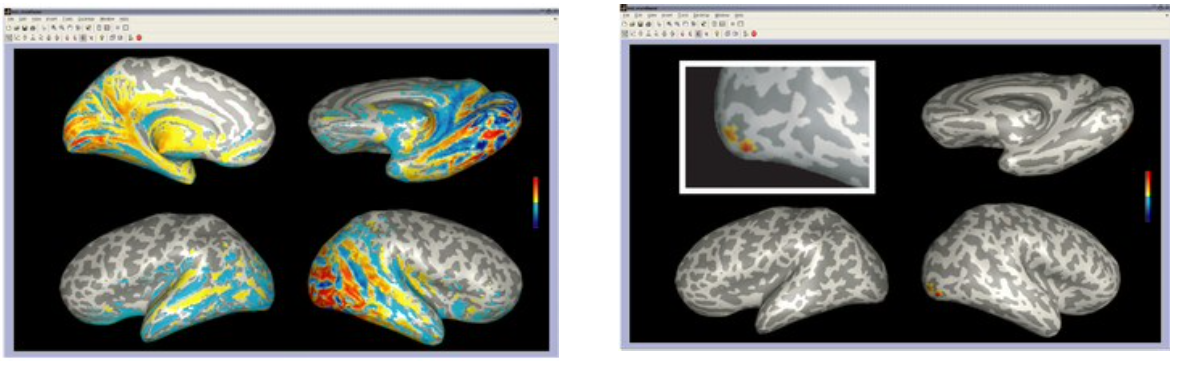
\includegraphics[width=0.8\linewidth]{image/dsm3}
		\caption{sLORETA (Left), Sparse Bayesian Learning (Right)}
	\end{figure}
\end{frame}
%
%\subsection{Temporal Characteristics}
%
%\begin{frame}
%\frametitle{Neural vs. Scalp activity}
%\begin{itemize}
%	\item Typical spiking behavior of a single neuron
%\end{itemize}
%	\begin{figure}
%		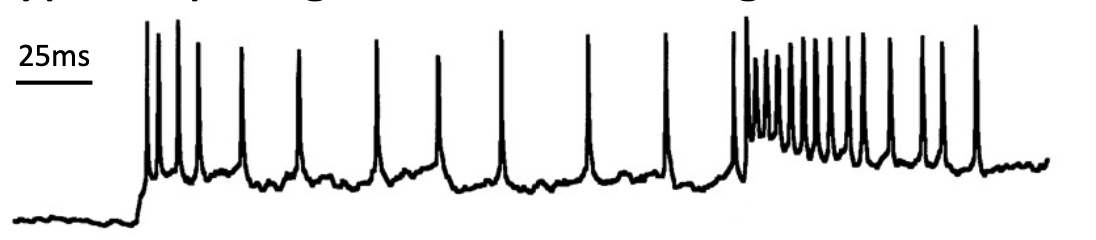
\includegraphics[width=0.7\linewidth]{image/spike}
%		\caption{Tsodkys, 1997)}
%	\end{figure}
%	\begin{itemize}
%	\item Typical signal measured at a scalp site
%\end{itemize}
%	\begin{figure}
%		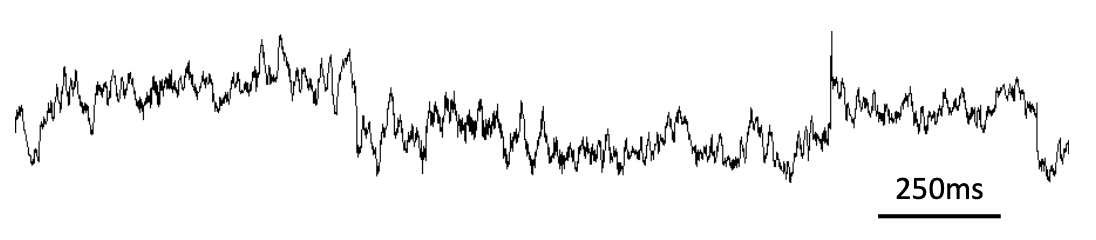
\includegraphics[width=0.7\linewidth]{image/real}
%		\caption{Tsodkys, 1997)}
%	\end{figure}
%\end{frame}
%
%
%
%\begin{frame}
%\frametitle{Oscillatory Processes}
%\begin{itemize}
%	\item EEG is permeated by oscillatory processes, such as the alpha rhythm (pictured)
%	\item Standard names for such rhythms are delta (0-4Hz), theta (4-7Hz), alpha (8-13Hz), beta(12-30Hz), and gamma(25-100Hz)
%\end{itemize}
%	\begin{figure}
%		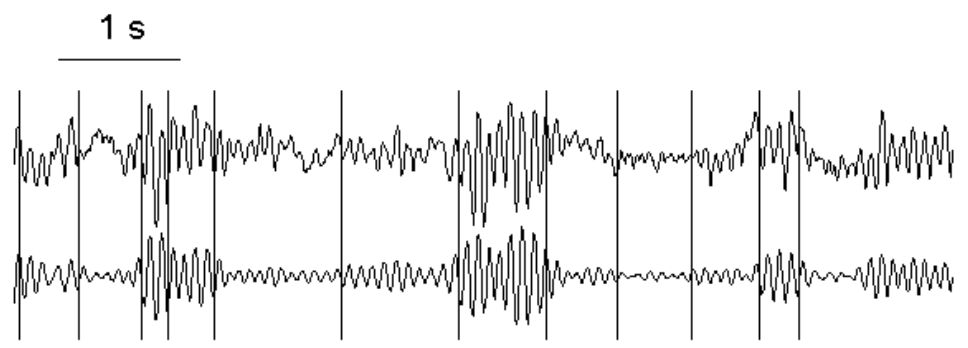
\includegraphics[width=0.8\linewidth]{image/op}
%		\caption{Kaplan et al., 2000}
%	\end{figure}
%\end{frame}  
%
%\begin{frame}
%\frametitle{Oscillatory Processes}
%\begin{itemize}
%	\item \textbf{Alpha}: Sensory areas (visual cortex, auditory cortex) and Motor areas (motor cortex) exhibit strong alpha-band oscillations when “idle” in most subjects
%	\item \textbf{Beta}: Motor cortex often generates also beta- band oscillations
%	\item \textbf{Theta}: Known to occur in “bursts” relative to events in certain brain areas (e.g. frontal midline, lateral frontal, ...)
%\end{itemize}
%\end{frame}

\subsection{Artifact Removal}

\begin{frame}
\frametitle{Non-Brain Artifacts}
\begin{itemize}
	\item Often far outscale the brain processes in the EEG (when present)
	\item \textbf{Internally} generated: neck, face, and eye muscles, eye dipoles, heart activity
\textbf{	\item Externally generated: 50/60Hz line noise, EM spikes from equipment
}	\item \textbf{Sensor}-related: DC offset drifts, cable sway, thermal noise, quantization noise
\end{itemize}
\end{frame}

\begin{frame}
\frametitle{Muscle Artifacts}
\begin{itemize}
	\item High-frequency / broadband, large amplitude
\end{itemize}
\begin{figure}
	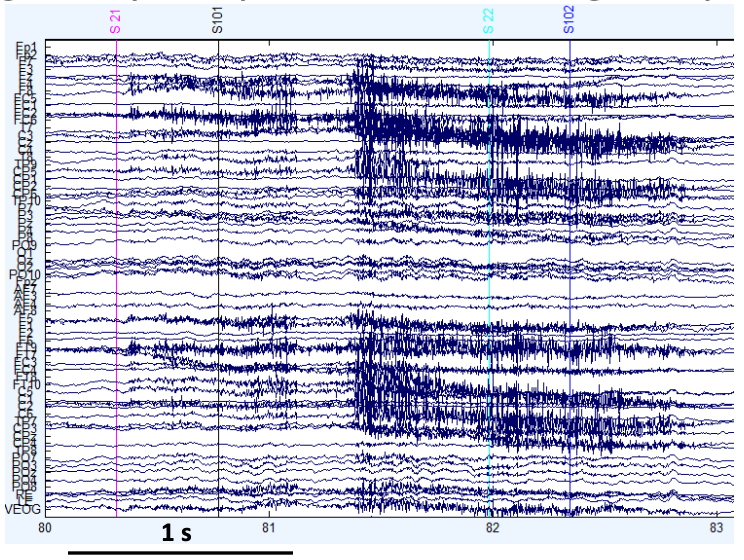
\includegraphics[width=0.6\linewidth]{image/emg}
	\caption{Muscle Artifacts}
\end{figure}
\end{frame}

\begin{frame}
\frametitle{Muscle Artifacts}
\begin{itemize}
	\item Scalp projections are spatially stereotyped
\end{itemize}
\begin{figure}
	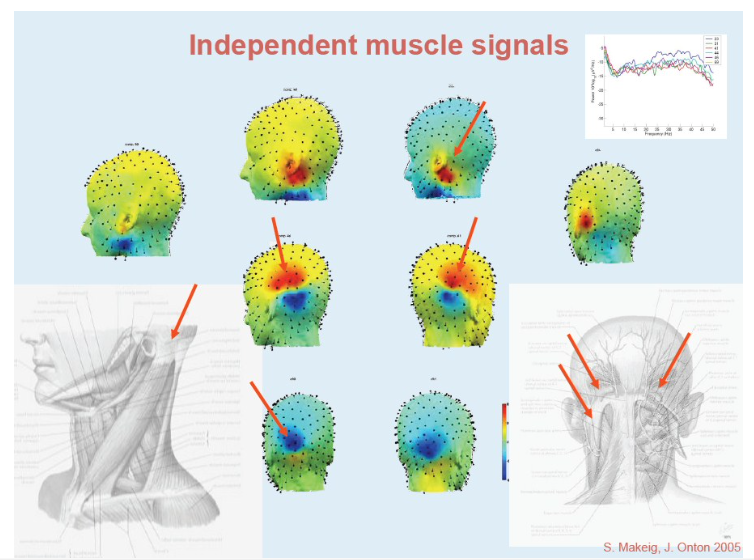
\includegraphics[width=0.6\linewidth]{image/emg2}
	\caption{Muscle Artifacts}
\end{figure}
\end{frame}

\begin{frame}
\frametitle{Eye Blinks}
\begin{itemize}
	\item Large low-frequency peak and rebound, mainly frontal
	\item Can also incurs non-linear effects in occipital cortex
\end{itemize}
\begin{figure}
	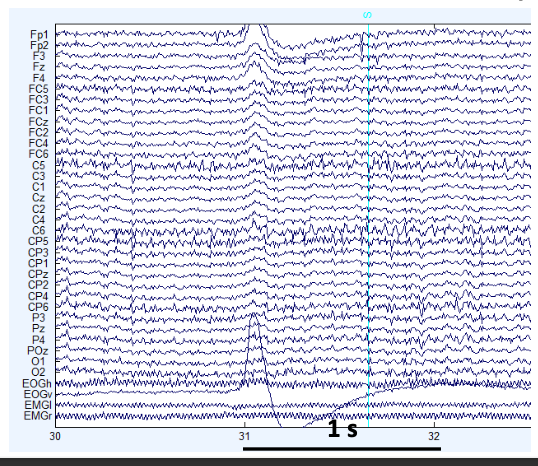
\includegraphics[width=0.5\linewidth]{image/eog}
	\caption{Eye Blinks Artifacts}
\end{figure}
\end{frame}

\begin{frame}
\frametitle{Bandpass Filters}
\begin{itemize}
	\item Easiest way to remove artifacts is simply to select only the frequency of interest	
\end{itemize}
\begin{figure}
	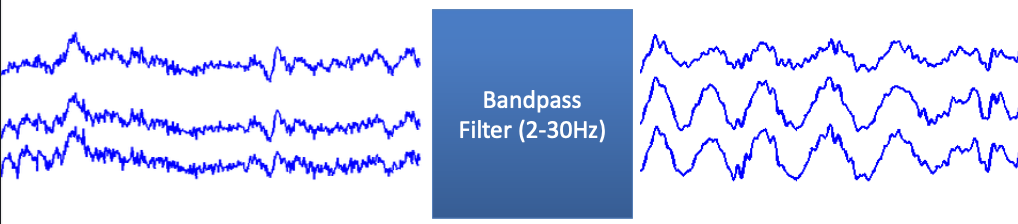
\includegraphics[width=0.8\linewidth]{image/spectral}
	\caption{Bandpass filter}
\end{figure}
\end{frame}
%
%\begin{frame}
%\frametitle{A Key Spectral Filters}
%\begin{itemize}
%	\item FIR (Finite Impuluse Reponse) Filter:
%\end{itemize}
%\begin{equation}
%	\mathcal{T} = y_i(n) = \sum_{k=0}^m b_k x_i (n-t)
%\end{equation}
%\begin{itemize}
%	\item Performs a convolution between signal and kernel
%	\item The trick lies on the coefficients ("kernel")$b_k$
%	\item Can implement any linear time-invariant spectral filter
%	\item Moving average is a special case
%\end{itemize}
%\end{frame}
%
%\begin{frame}
%\frametitle{Filter Implementations}
%\begin{figure}
%	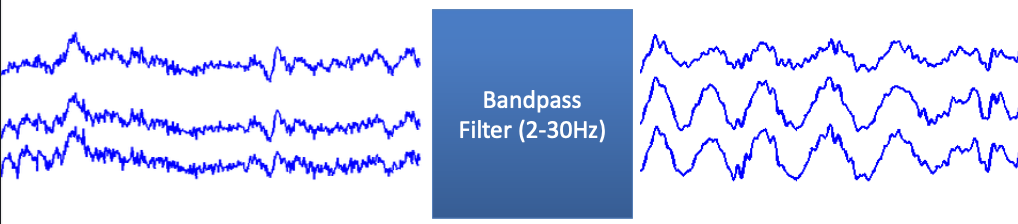
\includegraphics[width=0.8\linewidth]{image/spectral}
%	\caption{Filter implementations}
%\end{figure}
%\end{frame}
%
%\begin{frame}
%\frametitle{Bandpass vs. Fourier}
%\begin{itemize}
%	\item Fast Fourier transform does not extract any frequency bands. It only shows the frequency content of a given signal.
%	\item Bandpass filters on the hand eliminate some frequency content of a signal
%\end{itemize}
%\end{frame}

\begin{frame}
\frametitle{Independent Component Analysis}
\begin{figure}
	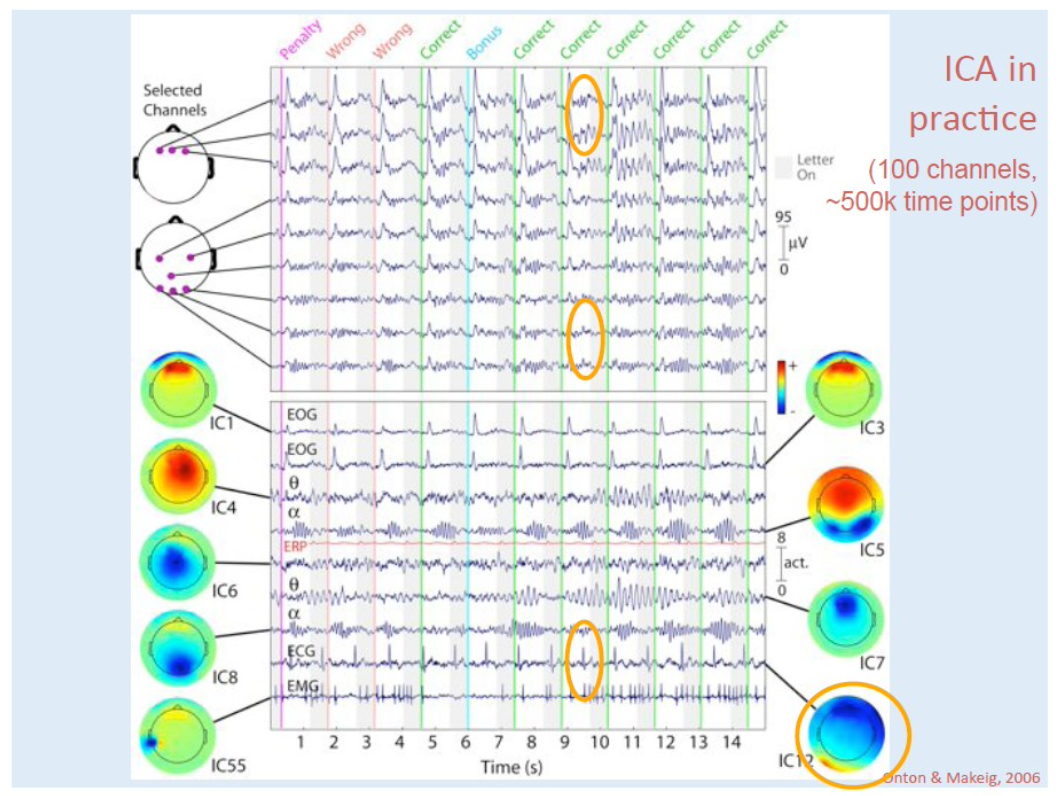
\includegraphics[width=0.7\linewidth]{image/ica}
	\caption{Onton and Makeig 2006}
\end{figure}
\end{frame}

\begin{frame}
\frametitle{Deep Neural Network}
\begin{figure}
	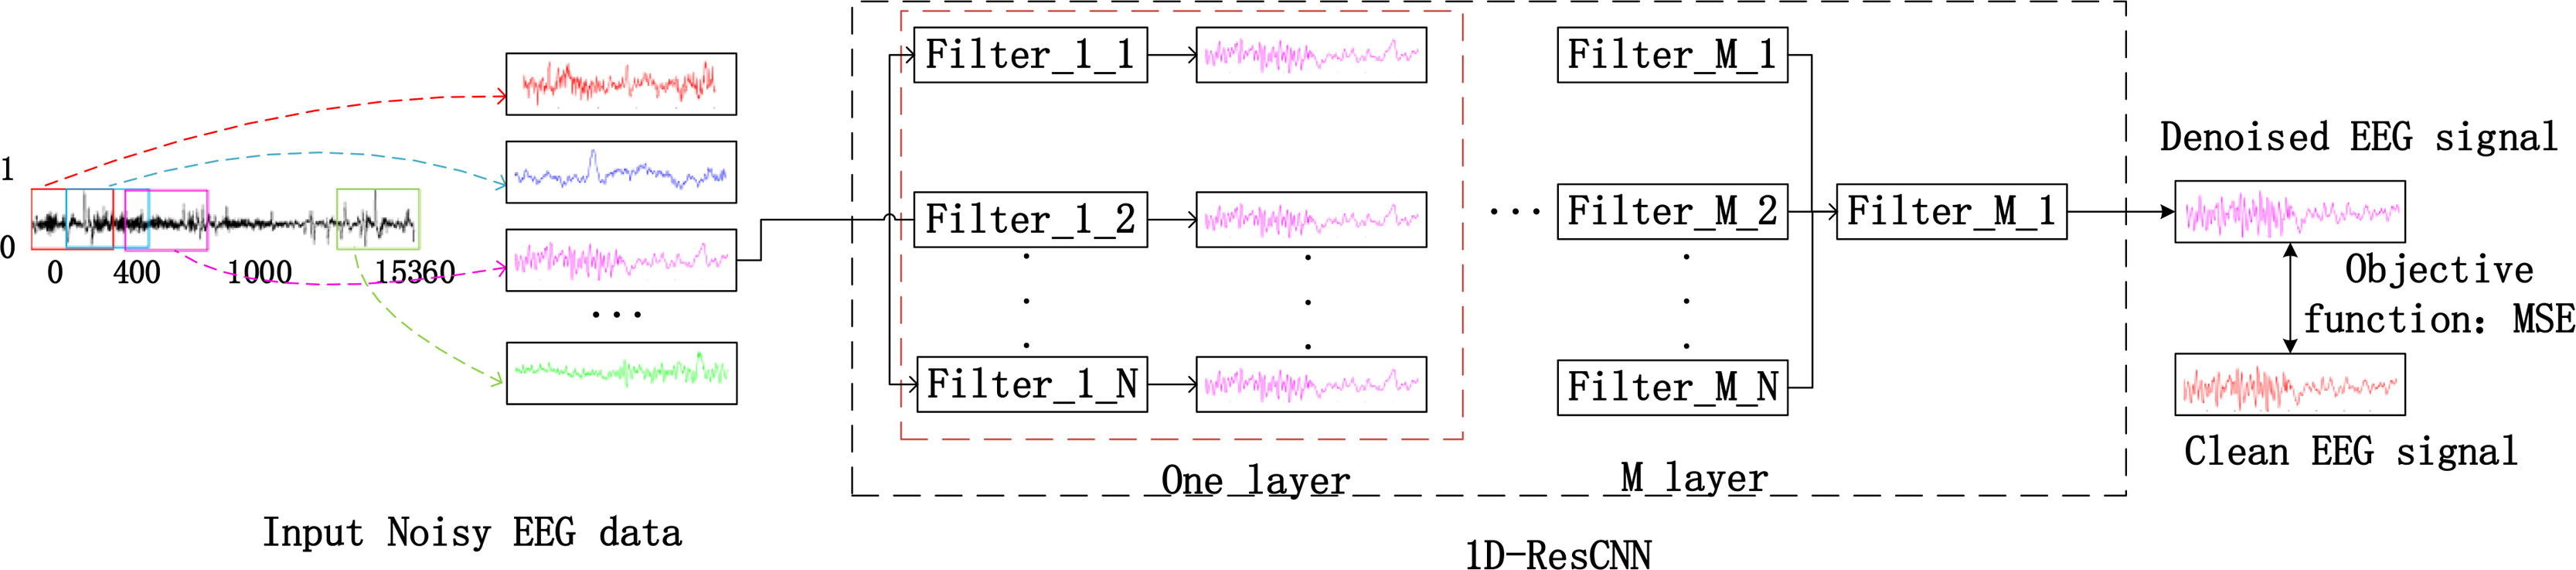
\includegraphics[width=0.9\linewidth]{image/resnet}
	\caption{\url{https://www.sciencedirect.com/science/article/abs/pii/S0925231220305944}}
\end{figure}
\end{frame}

\subsection{Other Niche Analyses}

\begin{frame}
\frametitle{Event-Related Coherence}
\begin{itemize}
	\item Event-Related Coherence between two signal components
\end{itemize}
\begin{figure}
	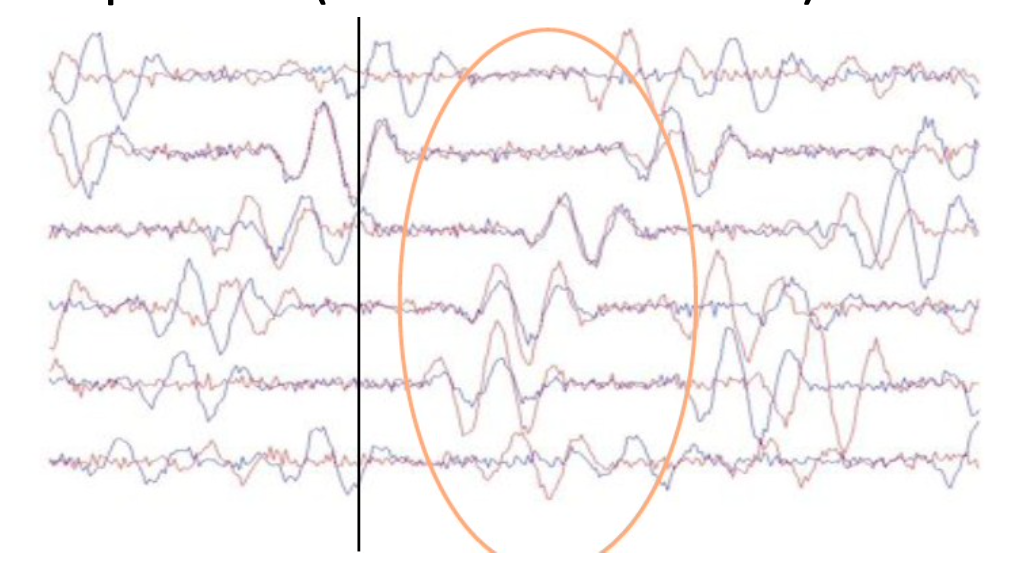
\includegraphics[width=0.7\linewidth]{image/erc}
	\caption{Makeig 2007}
\end{figure}
\end{frame}

\begin{frame}
\frametitle{Connectivity}
\begin{itemize}
	\item Sophisticated measure of interaction between multiple signals
	\item By getting the source estimates along the time, we can construct the connectivity plot
\end{itemize}
\begin{figure}
	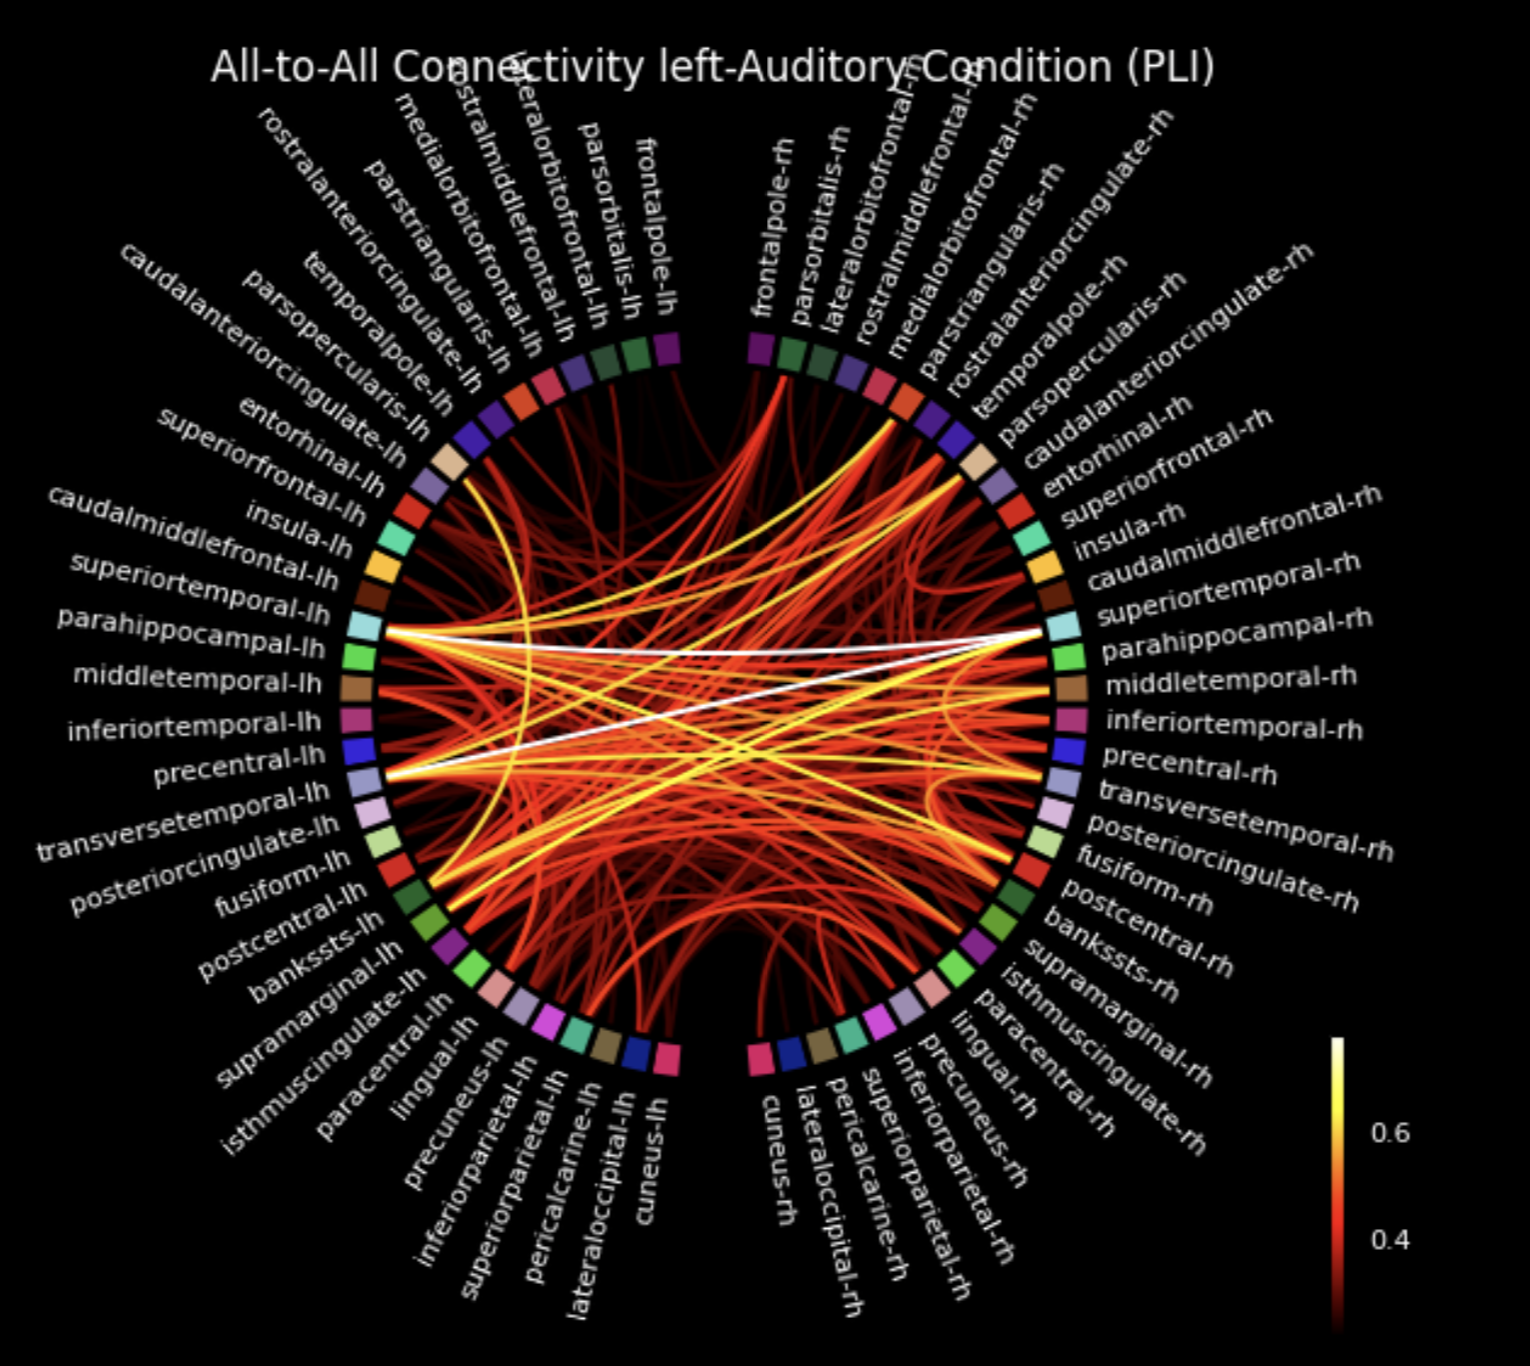
\includegraphics[width=0.4\linewidth]{image/connectivity2}
	\caption{Python MNE}
\end{figure}
\end{frame}

\section{In Action}

\begin{frame}
\frametitle{Measurement Sites}
\begin{itemize}
	\item Standardized location system (10-20 system)
	\item Saves a lot of hassle vs. custom labels
	\item Often defined in 8, 16, 32, and 64 channels
\end{itemize}
	\begin{figure}
		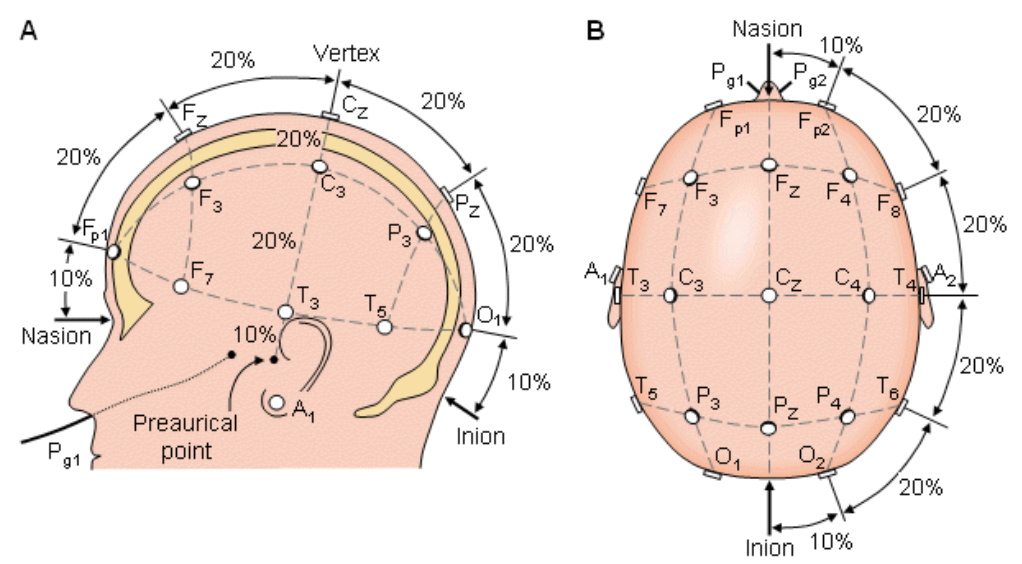
\includegraphics[width=0.7\linewidth]{image/10-20}
		\caption{International 10-20 system (Malmivuo and Plonsey, 1995)}
	\end{figure}
\end{frame}

\begin{frame}
\frametitle{Measurement Sites}
	\begin{figure}
		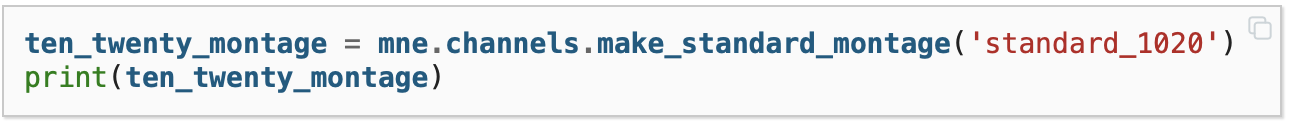
\includegraphics[width=0.7\linewidth]{image/montage}
	\end{figure}
		\begin{figure}
		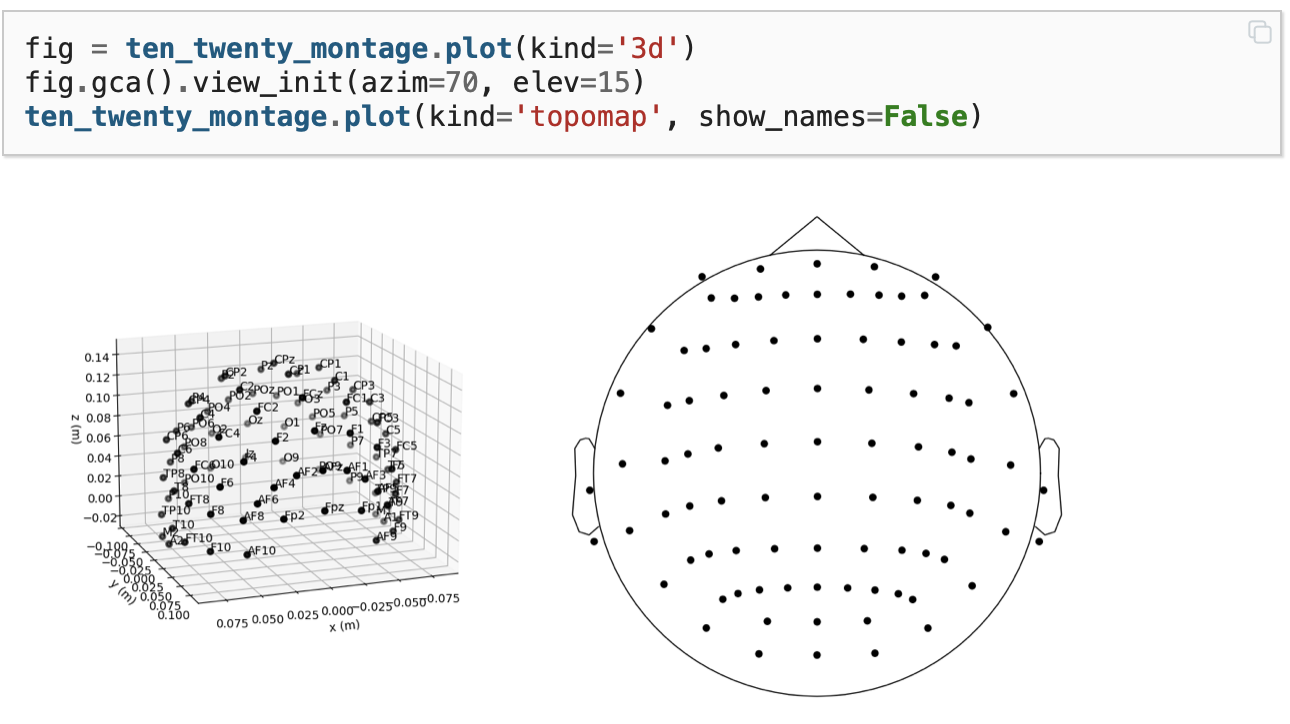
\includegraphics[width=0.7\linewidth]{image/montage2}
		\caption{Montage objects have a plot() method for visualization of the sensor locations in 3D; 2D projections are also possible by passing kind='topomap'}
	\end{figure}
\end{frame}

\begin{frame}
\frametitle{Where to put electrodes?}
\begin{itemize}
	\item Some notable large-scale brain features are the hemispheres, lobes, gyri and suci
	\item No nerves coming to frontal lobe thus it's less obvious what they do
\end{itemize}
	\begin{figure}
		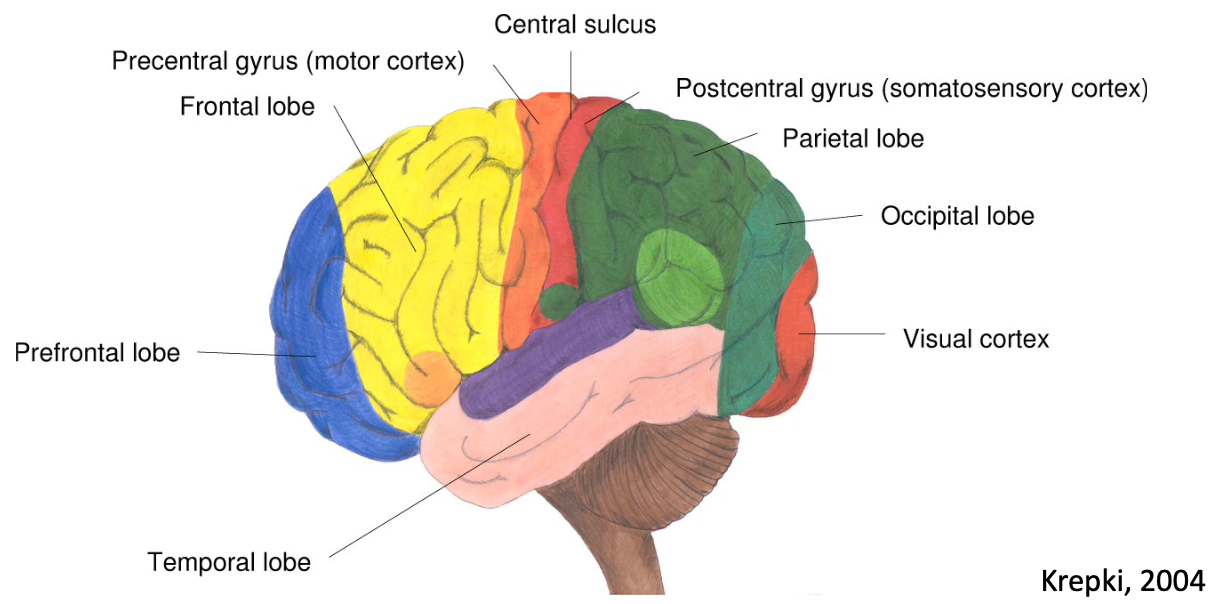
\includegraphics[width=0.7\linewidth]{image/structure}
		\caption{Major anatomical regions}
	\end{figure}
\end{frame}

\begin{frame}
\frametitle{Functional Mapping}
\begin{itemize}
	\item For most regions more or less well known functional associations exist - the motor cortex is one of the best examples
\end{itemize}
	\begin{figure}
		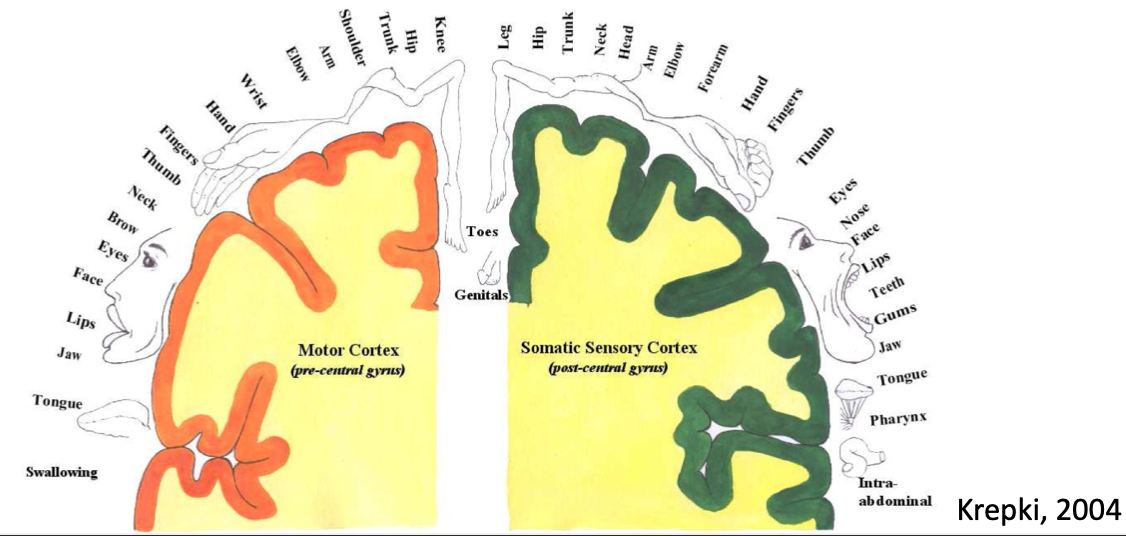
\includegraphics[width=0.7\linewidth]{image/motor}
		\caption{Homunculus: Functional mappings of the motor cortex}
	\end{figure}
\end{frame}

\begin{frame}
\frametitle{EEG Sensor Designs}
\begin{itemize}
	\item Most EEG systems are gel-based
	\item Nowadays mostly using active electrodes (i.e., with amplifiers)
\end{itemize}
\begin{figure}
	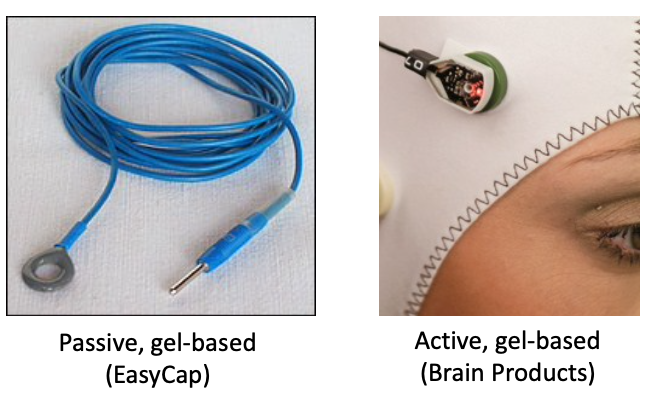
\includegraphics[width=0.7\linewidth]{image/sensor}
	\caption{EEG gel-based sensor}
\end{figure}
\end{frame}

\begin{frame}
\frametitle{EEG Sensor Designs}
\begin{itemize}
	\item Dry systems are emerging quickly
\end{itemize}
\begin{figure}
	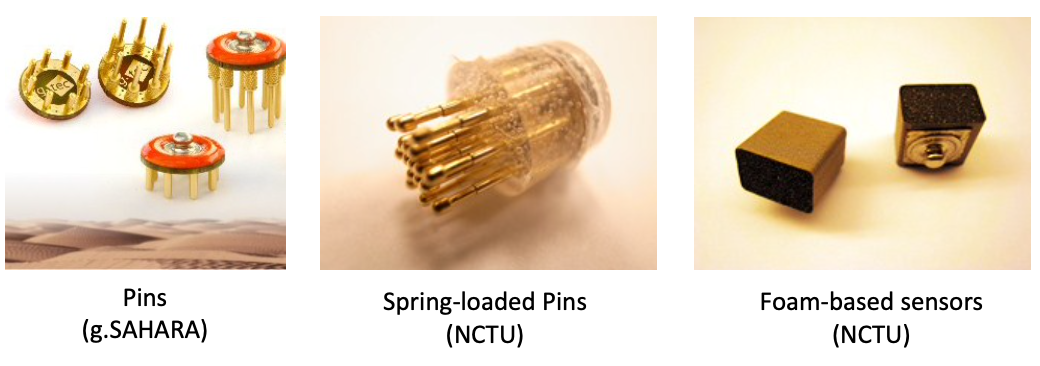
\includegraphics[width=0.7\linewidth]{image/sensor2}
	\caption{EEG dry-based sensor}
\end{figure}
\end{frame}

\begin{frame}
\frametitle{Digitization}
\begin{itemize}
	\item After amplification (e.g. 50000x), signal is low-pass filtered using an analog filter, then digitally sampled at fixed rate
\end{itemize}
\begin{figure}
	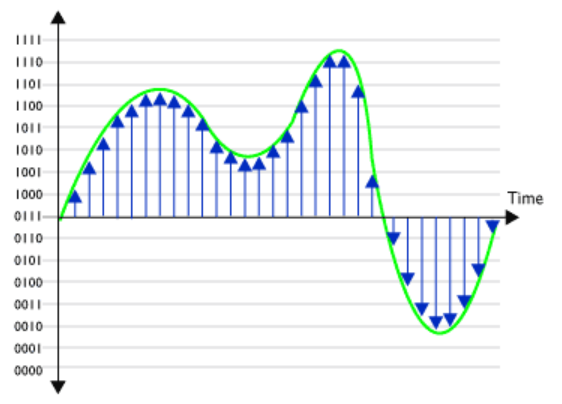
\includegraphics[width=0.7\linewidth]{image/digitalization}
	\caption{Digitization}
\end{figure}
\end{frame}

\begin{frame}
\frametitle{Sampling Theorem}
\begin{itemize}
	\item If the signal is band-limited below the Nyquist frequency B (i.e., contains no higher frequency than B), it can be exactly reconstructed using the interpolation function:
\end{itemize}
\begin{equation}
	g(t) = \frac{sin2\pi Bt}{2\pi Bt}
\end{equation}
\begin{equation}
	s(t) = \sum_{n=-\infty}^{\infty}s\left(\frac{n}{F_s}\right) g\left(\frac{t-n}{F_s}\right)
\end{equation}
\begin{itemize}
	\item The Nyquist Frequent is $\frac{1}{2}$ sampling rate
\end{itemize}
\end{frame}

\begin{frame}
\frametitle{OpenBCI connection}
\begin{figure}
	\includegraphics[width=0.6\linewidth]{image/openbci}
	\caption{Cyton with Daisy configuration.  The Y splitter (white) on SRB,  connecting to earlobe.  Another reference wire on BIAS (black), connecting to another earlobe.  Earlobe is used as reference because it has no muscles or neurons and therefore very low electrical signals. }
\end{figure}
\end{frame}

\begin{frame}
\frametitle{OpenBCI connection}
\begin{figure}
	\includegraphics[width=0.6\linewidth]{image/gold}
	\caption{Gold cup electrodes can be used to connect to other part of the body to the Cyton and Daisy board.   First scope the electrode paste into the electrode.    Then paste accordingly.}
\end{figure}
\end{frame}

\begin{frame}
\frametitle{OpenBCI connection}
\begin{figure}
	\includegraphics[width=0.8\linewidth]{image/GUI_Impedance}
	\caption{When the Ohm icon is toggled on, the board sends a small current through the selected channel to obtain the impedance value. For this reason, you won't be able to stream data on a channel and obtain the impedance value simultaneously.}
\end{figure}
\end{frame}

\begin{frame}
\frametitle{OpenBCI connection}
\begin{figure}
	\includegraphics[width=0.7\linewidth]{image/spectrogram}
	\caption{A dual spectrogram display which allows users to see changes in FFT data over time}
\end{figure}
\end{frame}

\begin{frame}
\frametitle{OpenBCI connection}
\begin{figure}
	\includegraphics[width=0.7\linewidth]{image/bandpower}
	\caption{One easy way to test the system is to ask users to close their eyes, the alpha should be low}
\end{figure}
\end{frame}

\begin{frame}
\frametitle{OpenBCI connection}
\begin{figure}
	\includegraphics[width=0.7\linewidth]{image/ssvep2}
	\caption{SSVEP widget}
\end{figure}
\end{frame}

\begin{frame}
\frametitle{OpenBCI connection}
\begin{figure}
	\includegraphics[width=0.7\linewidth]{image/emgwid}
	\caption{EMG widget:  if you relax, the value will be 0, and if you flex, the value will go to 1}
\end{figure}
\end{frame}

\begin{frame}
\frametitle{OpenBCI connection}
\begin{figure}
	\includegraphics[width=0.7\linewidth]{image/lsl}
	\caption{Lab Streaming Layer is a system for synchronizing streaming data for live analysis or recording.   LSL is a good way to send your OpenBCI stream to applications like Python.}
\end{figure}
\end{frame}

\begin{frame}
\frametitle{Example: Using EMG to stop/start music}
\begin{figure}
	\includegraphics[width=0.7\linewidth]{image/emgplacement}
	\caption{Connect to top N1pin and bottom N1pin for measuring potential difference.  The elbow is connected to the bottom AGND pin for reference.}
\end{figure}
\end{frame}

\begin{frame}
\frametitle{Example: Using EMG to stop/start music}
\begin{figure}
	\includegraphics[width=0.7\linewidth]{image/lsl2}
	\caption{Turn on the EMG and LSL widgets.}
\end{figure}
\end{frame}

\begin{frame}
\frametitle{Example: Using EMG to stop/start music}
\begin{figure}
	\includegraphics[width=0.7\linewidth]{image/emgcontrol}
	\caption{EMG to start/stop music}
\end{figure}
\end{frame}

%\section{Signal Processing}
%
%\subsection{Role of Signal Processing}
%
%\begin{frame}
%\frametitle{BCI Theory}
%\begin{itemize}
%	\item BCI leverages theory from a wide range of fields (Signal Processing, Machine Learning, Statistics, Neuroscience, Control Theory, Information Theory, ...)
%	\item A given BCI may be understood from the vantage point of any of these theories
%	\item But no single theory conveniently describes all aspects of a BCI
%\end{itemize}
%\end{frame}
%
%\begin{frame}
%\frametitle{Signal Processing}
%\begin{itemize}
%	\item \textbf{Digital Signal Processing} is concerned with systems (a.k.a. filters) that transform one signal into another
%	\item \textbf{Linear Time-Invariant (LTI) Systems}, including Spectral filters and their optimal design are one of the most developed areas
%	\item \textbf{Statistical Signal Processing} and \textbf{Adaptive Filtering} are among the advanced areas (Kalman Filter, etc., recursive least-squares)
%	\item \textbf{Sparse Signal Processing} (e.g., sparse recovery and compressive sensing) is a new branch with application to BCIs
%\end{itemize}
%\end{frame}
%
%\begin{frame}
%\frametitle{Signal Processing}
%\begin{itemize}
%	\item A signal is a mapping from an index set (here discrete time) onto vectors (multichannel samples)
%	\item From the point of view of Signal Processing, a BCI transduces the input signal $x(n)$ (for example EEG) into a control signal $y(n)$
%	\item It is defined by a transformation rule $T$
%\end{itemize}
%\begin{equation}
%	y(n) = \mathcal{T}[x(n)]
%\end{equation}
%\end{frame}
%
%\begin{frame}
%\frametitle{Important System Types}
%\begin{itemize}
%	\item A system is called \textbf{static} if the value $y(n)$ at any sample $n$ depends only on $x(n)$, otherwise \textbf{dynamic}.
%	\item A system is called \textbf{causal} if the output $y(n)$ at any time $n$ only depends on values of $x(m)$ for $m \leq n$, otherwise \textbf{non-causal}.
%	\item A system is called \textbf{time-invariant} if $y(n) = T[x(n)]$ implies that $y(n-k) = T[x(n-k)]$ for every time shift $k$, otherwise \textbf{time-variant}.
%	\item A system is called \textbf{linear} if the equation $T[a_1x_1(n) + a_2x_2(n)] = a_1T[x_1(n)] + a_2T[x_2(n)]$ holds for all
%inputs $x_1(n)$ and $x_2(n)$ and all constants $a_1$ and $a_2$, otherwise nonlinear.
%\end{itemize}
%\end{frame}
%
%\begin{frame}
%\frametitle{BCIs Viewed as Filters}
%\begin{itemize}
%	\item Since BCIs are operated in real time, they are always \textbf{causal} systems
%	\item BCIs usually perform temporal filtering, and are therefore \textbf{dynamic}
%	\item Some BCIs are \textbf{time-invariant}, but adaptive BCIs are not
%	\item Simple BCIs are \textbf{linear}, but the vast majority is not
%	\item Since their output is needed at a much lower sampling rate (0.1-60Hz) than the input (250-1000Hz), they are technically \textbf{multi-rate} systems
%\end{itemize}
%\end{frame}
%
%\begin{frame}
%\frametitle{BCI Components as Filters}
%\begin{itemize}
%	\item BCI components are conveniently described as filters – more so than the entire system itself
%	\item This gives rise to several key categories of filter components
%\end{itemize}
%\begin{figure}
%	\includegraphics[width=0.8\linewidth]{image/filter}
%	\caption{Filter components}
%\end{figure}
%\end{frame}
%
%\subsection{Major Filter Classes}
%
%\begin{frame}
%\frametitle{Static Filters}
%\begin{itemize}
%	\item Signal \textbf{squaring}: static system, useful step in calculating the variance of the signal
%\end{itemize}
%\begin{equation}
%	\mathcal{T} = y_i(n) = x_i(n)^2
%\end{equation}
%\begin{figure}
%	\includegraphics[width=0.8\linewidth]{image/square}
%	\caption{Signal Squaring}
%\end{figure}
%\begin{itemize}
%	\item \textbf{Logarithm} - allows simple numbers to represent large variations in signal levels - very useful in calculating system gains and losses
%\end{itemize}
%\begin{equation}
%	\mathcal{T} = y_i(n) = \log x_i(n)
%\end{equation}
%\end{frame}

%
%
%\subsubsection{Temporal Filters}
%
%\begin{frame}
%\frametitle{Temporal Filters}
%\begin{itemize}
%	\item Transform a multi-channel signal $X(n)$ such that each channel $y_i(n)$ in $Y(n)$ depends only on the channel $x_i(n)$
%	\item They are conceptually orthogonal to spatial filters
%	\item Examples include time windowing, wavelet transform, etc.
%	\item Special case: Spectral filters
%\end{itemize}
%\end{frame}
%
%\begin{frame}
%\frametitle{Temporal Filters}
%\begin{itemize}
%	\item \textbf{Moving Average}: Effectively a smoothing operator and in fact a simple example of spectral filter
%\end{itemize}
%\begin{equation}
%	\mathcal{T} = y_i(n) = \frac{1}{m} \sum_{k=0}^{m-1}x_i(n-k)
%\end{equation}
%\begin{figure}
%	\includegraphics[width=0.8\linewidth]{image/ma}
%	\caption{Moving average}
%\end{figure}
%\end{frame}
%
%\subsubsection{Spectral Filters}
%
%\begin{frame}
%\frametitle{Spectral Filters}
%\begin{itemize}
%	\item Temporal filters that are designed for their effects on the spectrum of the signal
%	\item \textbf{Spectrum} of a signal:  a representation of the signal as a sum of $N$ sinusoidal components,
%\end{itemize}
%\begin{equation}
%	s(n) = \sum_{k=1}^N A_k sin(k n T + \phi_k)
%\end{equation}
%\hspace{20pt} where $A_k$ is the amplitude of each sinusoid and $\phi_k$ is the phase offset
%\end{frame}
%
%\begin{frame}
%\frametitle{Spectral Filters}
%\begin{itemize}
%	\item An equivalent (more common) representation is the Fourier Series representation ($j$ is the imaginary number, $k$ is the frequency)
%\end{itemize}
%\begin{equation}
%	s(n) = \sum_{k=0}^{N-1} A_k e^{j2\pi kn / N}
%\end{equation}
%\hspace{20pt} where $A_k$ is now complex-valued representing both  amplitude and \hspace{20pt} phase
%\begin{itemize}
%	\item This relies on the Euler formula
%\end{itemize}
%\begin{equation}
%	e^{\pm j\phi} = \cos \phi \pm j \sin \phi
%\end{equation}
%\end{frame}



%\begin{frame}
%\frametitle{Minimum-Phase Filter Design}
%\begin{itemize}
%	\item Linear-Phase Lowpass (uniform lag):
%\end{itemize}
%\begin{figure}
%	\includegraphics[width=0.6\linewidth]{image/phase1}
%\end{figure}
%\begin{itemize}
%	\item Minimum-Phase Lowpass (minimal lag)
%\end{itemize}
%\begin{figure}
%	\includegraphics[width=0.6\linewidth]{image/phase2}
%\end{figure}
%\end{frame}
%
%\subsection{Example: A Simple Neurofeedback BCI}
%
%\begin{frame}
%\frametitle{A Simple Neurofeedback BCI}
%\begin{itemize}
%	\item Feedback the amplitude of a brain idle oscillation (e.g., 10Hz alpha for relaxation) to the user
%\end{itemize}
%\begin{figure}
%	\includegraphics[width=0.7\linewidth]{image/neurofeedback}
%	\caption{Spectral filters, static filters, temporal filters, and static filters}
%\end{figure}
%\end{frame}

\section{Deep Learning Architectures}

\subsection{Basic CNN}

\begin{frame}
\frametitle{Basic CNN}
\begin{figure}
	\includegraphics[width=0.35\linewidth]{image/basic}
	\caption{\url{https://www.sciencedirect.com/science/article/pii/S2213158219300348}}
\end{figure}
\end{frame}

\subsection{EEGNet}

\begin{frame}
\frametitle{EEGNet (2018)}
\begin{figure}
	\includegraphics[width=0.7\linewidth]{image/eegnet}
	\caption{\url{https://arxiv.org/abs/1611.08024}}
\end{figure}
\end{frame}

\subsection{Cross-Modal Learning}

\begin{frame}
\frametitle{Cross-Modal Learning (2020)}
\begin{figure}
	\includegraphics[width=0.65\linewidth]{image/crossmodal}
	\caption{\url{https://www.sciencedirect.com/science/article/abs/pii/S0031320319303863}}
\end{figure}
\end{frame}


%\subsection{Prediction Function Notion}
%
%\begin{frame}
%\frametitle{Functional Form}
%\begin{itemize}
%	\item The functional form is arbitrary,  where $X$ is a multichannel time series data,  where you can slide a window to query for a particular time you are interested,  for example
%\end{itemize}
%\begin{equation}
%	y = sign(var(WX) + b)
%\end{equation}
%\begin{itemize}
%	\item The mapping involves unknown parameters, here $W$ and $b$
%	\item Note: Functional form is the inverse mapping!
%\end{itemize}
%\begin{figure}
%	\includegraphics[width=0.7\linewidth]{image/function}
%	\caption{Relationship between observation (X) and output (y)}
%\end{figure}
%\end{frame}
%
%\begin{frame}
%\frametitle{Core Ingredient: Spatial Filter}
%\begin{itemize}
%	\item Linear inverse of volume conduction effect
%\end{itemize}
%\begin{equation}
%	X = AS       \text{    (forward)}
%\end{equation}
%\begin{equation}
%	S = WX \text{      (inverse)}
%\end{equation}
%\begin{figure}
%	\includegraphics[width=0.4\linewidth]{image/volume}
%	\caption{The inverse relationship}
%\end{figure}
%\end{frame}
%
%\begin{frame}
%\frametitle{Full Examples}
%\begin{itemize}
%	\item Inverse mapping from filtered source time courses to latent cognitive state, e.g., :
%\end{itemize}
%\begin{equation}
%	y = \theta vec(WX) + b    \text{    (linear)}
%\end{equation}
%\begin{equation}
%	y = \theta vec(|(WX)T|) + b    \text{    (nonlinear)}
%\end{equation}
%\end{frame}
%
%\begin{frame}
%\frametitle{Neurofeedback BCI in Functional Style}
%\begin{itemize}
%	\item Performed as a mapping of a sliding window $X$ onto the output $y$
%\end{itemize}
%\begin{equation}
%	f(X) = y = \log var(XT)
%\end{equation}
%\begin{itemize}
%	\item $T$ implements a temporal filter, written as a matrix multiplication (each = shifted filter kernel)
%\end{itemize}
%\end{frame}
%
%\begin{frame}
%\frametitle{In Comparison...}
%\begin{itemize}
%	\item Main \textbf{drawback} of the pure mathematical form compared to the signal processing approach:
%	\begin{itemize}
%		\item The entire input window $X$ is re-processed for each desired output value $y$
%		\item Especially bad if the window $X$ moves only by a few samples between evaluations of $f$
%		\item In contrast, most signal processing methods are incremental or recursive (e.g., FIR or IIR)
%	\end{itemize}
%	\item Main \textbf{benefit} is the relative conceptual simplicity
%\end{itemize}
%\end{frame}
%
%\begin{frame}
%\frametitle{In Combination}
%\begin{itemize}
%	\item Both frameworks are complementary, rather than contradictory, and are in practice often used in combination
%\end{itemize}
%\begin{figure}
%	\includegraphics[width=0.8\linewidth]{image/combined}
%\end{figure}
%\end{frame}
%
%\begin{frame}
%\frametitle{Neurofeedback Using the Combined Approach}
%\begin{itemize}
%	\item Computationally costly spectral filtering is done in the signal processing portion
%	\item Lightweight predictive mapping is done at lower rate in the functional portion
%\end{itemize}
%\begin{figure}
%	\includegraphics[width=0.8\linewidth]{image/combined2}
%\end{figure}
%\end{frame}

\section{Good Resources}

\begin{frame}
\frametitle{Good Resources}
\footnotesize
\begin{itemize}
	\item Use \textbf{Python MNE} - is made by neuroscientists.  Documentation is also VERY well written.  They have (1) source estimation, (2) machine learning, (3) connectivity,  (4) awesome data visualization modules.   You will learn A LOT of neuroscience here.
	\item Although we did not use \textbf{MATLAB},  it has many good tutorials that will allow us to better understand how EEG works - \url{https://sccn.ucsd.edu/eeglab/index.php}
	\item Use \textbf{LSL} protocol with  \textbf{pyOpenBCI (python way)} or \textbf{OpenBCI GUI (GUI way)} to acquire data from the OpenBCI board.  
	\item Use \textbf{pygame}, \textbf{tkinter} or \textbf{javascript} if you want to make BCI application.  You have to use \textbf{threads} a lot so learn it.
	\item EEG \textbf{datasets}:  \url{https://github.com/meagmohit/EEG-Datasets}
	\item Best \textbf{youtube} channel for learning EEG - Mike X Cohen - \url{https://www.youtube.com/channel/UCUR_LsXk7IYyueSnXcNextQ}.   Our lab also has his book - \textbf{Analyzing Neural Time Series Data}.
	\item Another easy-to-read yet very good book is \textbf{Practical Approach to Electroencephalography} by Libenson.   Once you learn it, you can read \textbf{Rowan's Primer of EEG} (our lab also has it) which teaches you how to read EEG.
	\item Read \textbf{EEGNet} and \textbf{EEG-ChannelNet} if you are interested in deep learning + EEG
\end{itemize}
\end{frame}

\section{Future Research}

\begin{frame}
\frametitle{Future Research}
\footnotesize
The key questions in BCI remains unchanged and is still in the \textbf{infancy} stage.  The problem remains \textbf{unroboust accuracy}, \textbf{impracticality} due to many restrictions (e.g., many artifacts,  many variations in users),  does not really know what is \textbf{EEG} (e.g., where does it come from, what different features mean).   Here are some topics I often come across in recent years.
\begin{itemize}
	\item \textbf{Mobile} real-time EEG
	\item \textbf{Feature} Extraction (e.g., functional connectivity)
	\item \textbf{Fusion} model (e.g., LSTM + GCNN)
	\item \textbf{Artifact Removal / Source Localization}
	\item \textbf{Multimodal} EEG + other sources of input (e.g., fNIRS, facial, EMG, EKG)
	\item \textbf{One shot learning} from few training data (e.g., only 1 minute of EEG recordings! or only 1 electrode!)
	\item \textbf{Participant independent }model
	\item \textbf{Cross-modal learning }- EEG $\leftrightarrow$ audio/image/text
	\item \textbf{Data Augmentation}
	\item Understanding the underlying \textbf{neural processes }via EEG
\end{itemize}
\end{frame}


\begin{frame}
\Huge{\centerline{Questions}}
\end{frame}

%----------------------------------------------------------------------------------------

\end{document} 
